% =============================================================
% Section 3: Methods
% =============================================================
\section{Methods}\label{sec:methods}

We consider a forward Schwarzschild PINN, a Schwarzschild hFNO and a
Kerr hFNO. The forward PINN approximates one solution of the Zerilli
initial-boundary-value problem by minimising the equation, initial-data
and boundary-condition residuals. The two hFNOs are trained separately
on Schwarzschild mass and initial-data configurations and on Kerr spin
and initial-pulse configurations. For each configuration, the
finite-difference solver first computes a coarse-grid solution, after
which an FNO returns an additive correction on the output grid. QNM
parameters are extracted from the Schwarzschild waveform at the fixed
code coordinate $\xq=10$ and from the Kerr waveform at $\scri$.
For the canonical $M=1$ configuration, $\xq=10\,M$. The Schwarzschild
analysis uses M1--M5, while the Kerr analysis also uses estimators
defined directly for a complex waveform.

\begin{table}[!htbp]
\centering
\caption{Training configurations for the forward PINN and
Schwarzschild hFNO. All learning rates are $10^{-3}$; hFNO weight
decay is $10^{-6}$.}
\label{tab:train-config}
\footnotesize
\setlength{\tabcolsep}{5pt}
\begin{tabular}{@{}lcc@{}}
\toprule
 & Forward PINN & Schwarzschild hFNO \\
\midrule
Parameters & $4{,}521$ & $1.13\times 10^{6}$ \\
Optimiser  & Adam${\to}$L-BFGS & AdamW \\
Budget     & $10^{4} + 3{\times}10^{4}$ it. & $100$ ep. \\
Batch size & full & $8$ \\
Precision  & \texttt{float64} & \texttt{float32} \\
\bottomrule
\end{tabular}
\end{table}

% --------------------------------------------------------------
\subsection{Schwarzschild Zerilli problem}
\label{sec:fwd-problem}

The canonical Schwarzschild forward problem is the Zerilli equation
Eq.~\eqref{eq:zerilli} with the polar potential
$V_{\ell}^{\mathrm{Z}}$ of Eq.~\eqref{eq:V-zerilli}, evaluated at
$\ell=2$ and $M=1$ on the numerical domain
$x\in[-50,150]\,M$ and $t\in[0,50]\,M$. We use
outgoing Gaussian initial data
\begin{equation}
  \Phi(x,0) = A_0\,\exp\!\left[-\frac{(x-x_0)^2}{\sigma_0^2}\right],
  \qquad
  \partial_t \Phi(x,0) = -\partial_x \Phi(x,0)
  = \frac{2(x-x_0)}{\sigma_0^2}\,\Phi(x,0),
  \label{eq:ic}
\end{equation}
with $A_0 = 1$, $x_0 = 4\,M$ and $\sigma_0 = 5\,M$. This choice
enforces the outgoing flat-space condition
$(\partial_t+\partial_x)\Phi=0$ at $t=0$, so the initial packet
propagates towards spatial infinity before scattering from the
Zerilli potential. It differs only in the initial velocity profile
from the setup of \citet{Patel2024pinn}, while retaining their
amplitude, centre and width. At the finite radial boundaries
$x=x_{\min}$ and $x=x_{\max}$, we impose the first-order Sommerfeld
conditions
\begin{equation}
  (\partial_t - \partial_x)\Phi\bigl|_{x=x_{\min}} = 0, \qquad
  (\partial_t + \partial_x)\Phi\bigl|_{x=x_{\max}} = 0,
  \label{eq:bc-sommerfeld}
\end{equation}
These are the finite-domain outgoing conditions used by
\citet{Patel2024pinn}. They approximate ingoing radiation at the
horizon side and outgoing radiation at the outer boundary, rather
than the frequency-domain QNM eigenvalue conditions imposed at
$x\to\pm\infty$. The characteristic travel times from the packet
centre to the two boundaries are
\begin{equation}
  t_{R} = x_{\max} - x_0 = 146\,M, \qquad
  t_{L} = x_0 - x_{\min} = 54\,M,
  \label{eq:bc-arrival}
\end{equation}
Both times exceed the PINN evaluation window. The PINN boundary losses
therefore enforce the Sommerfeld conditions outside the domain of
dependence of the observer waveform over $0\leq t\leq50\,M$, while the
FD reference is insensitive to the boundaries over this interval.

The Zerilli reference field (Fig.~\ref{fig:waveform-3d}) is computed
with a method-of-lines finite-difference (FD) scheme using second-order centred
spatial differences, second-order one-sided boundary closures and
fourth-order Runge--Kutta time stepping, using $\Delta x = 0.2\,M$
and $\Delta t = 0.1\,M$. It is used as the numerical reference for
the Zerilli PINN field errors and as the finite-difference waveform
used to evaluate the QNM estimators. The Leaver values
$M\omega_0^R = 0.3737$,
$\tau_0/M = 11.241$ (fundamental) and $M\omega_1^R = 0.3467$,
$\tau_1/M = 3.651$ (first overtone) of Eq.~\eqref{eq:qnm-ref}
are used for percentage-error reporting.
The Regge--Wheeler reproduction uses the same domain, initial data,
boundary conditions, FD scheme and extraction protocol with
$V_{\ell}^{\mathrm{Z}}$ replaced by the axial Regge--Wheeler
potential. The later Schwarzschild extensions use the Zerilli
equation. The Regge--Wheeler and Zerilli equations have the same QNM
spectrum.

\begin{figure}[!htbp]
\centering
\begin{minipage}[t]{0.49\textwidth}
  \centering
  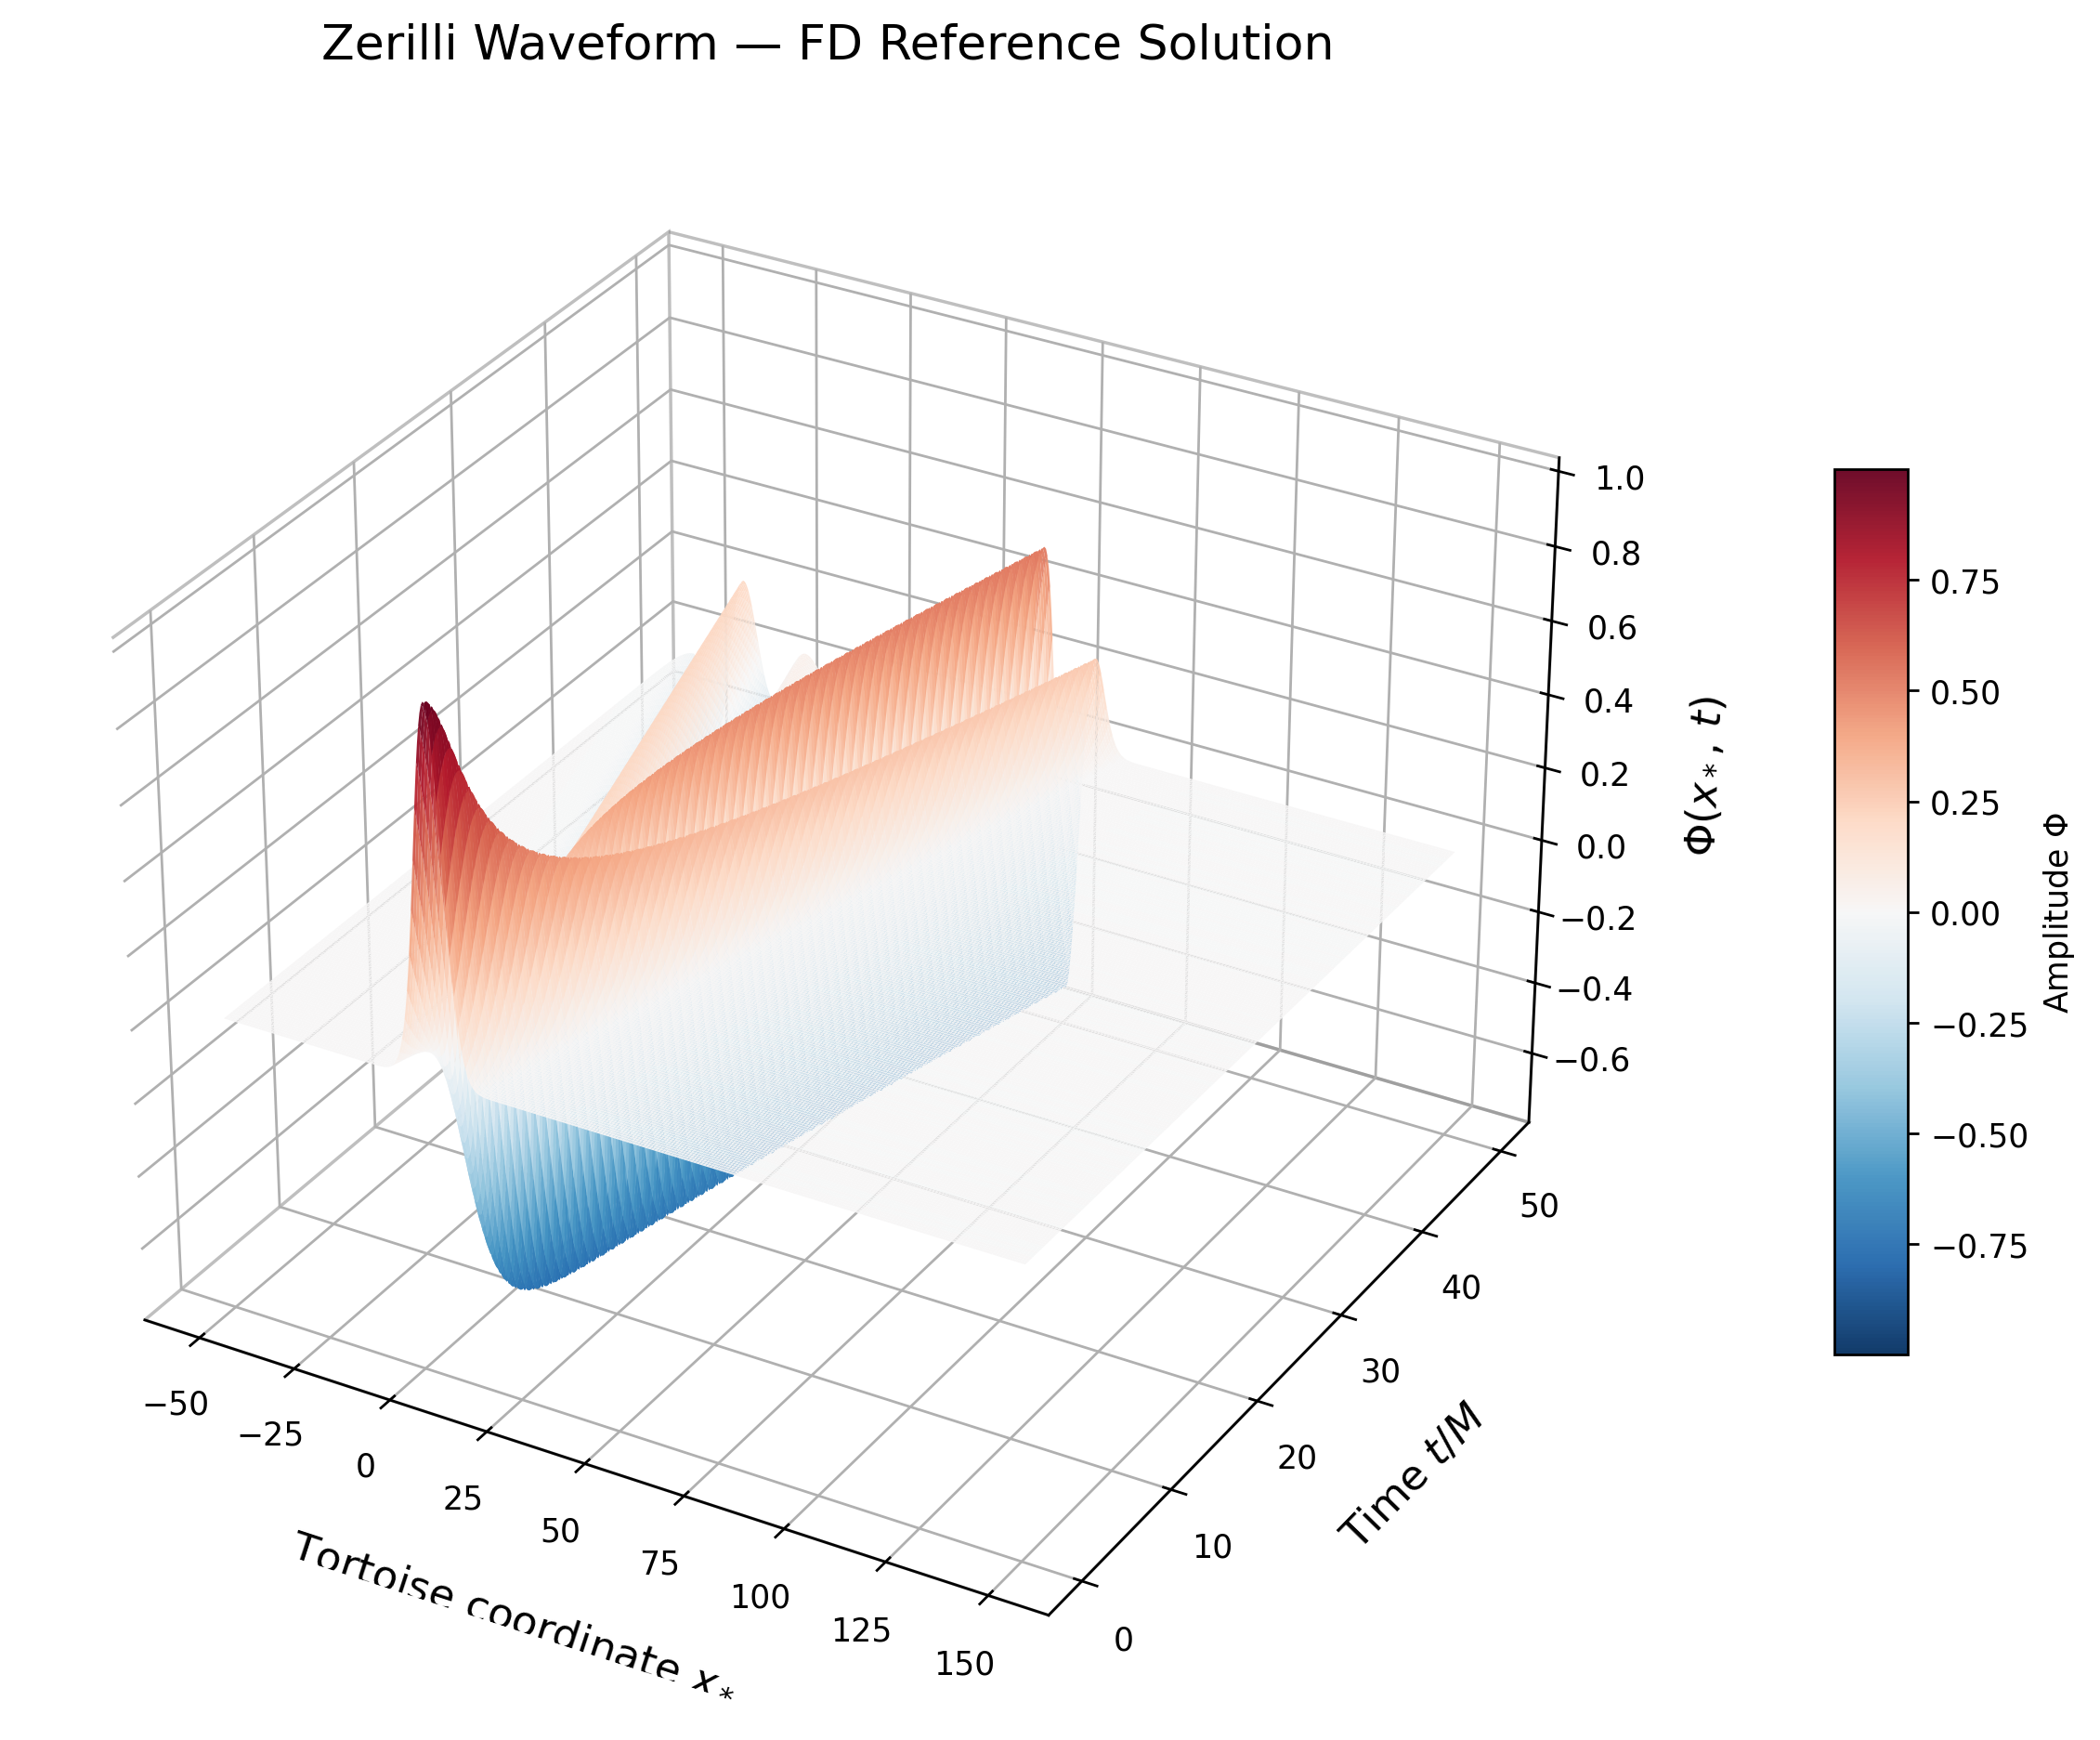
\includegraphics[width=\linewidth]{../outputs/pinn/waveform_3d_full.png}
  \subcaption{Full domain $x \in [-50, 150]\,M$, $t \in [0, 50]\,M$.
  The right-moving free pulse from the outgoing initial condition
  is visible as the diagonal ridge propagating to the right (towards
  infinity); the left-moving ridge towards the horizon is the
  back-scattered component generated by the photon-sphere barrier.}
  \label{fig:waveform-3d-full}
\end{minipage}\hfill
\begin{minipage}[t]{0.49\textwidth}
  \centering
  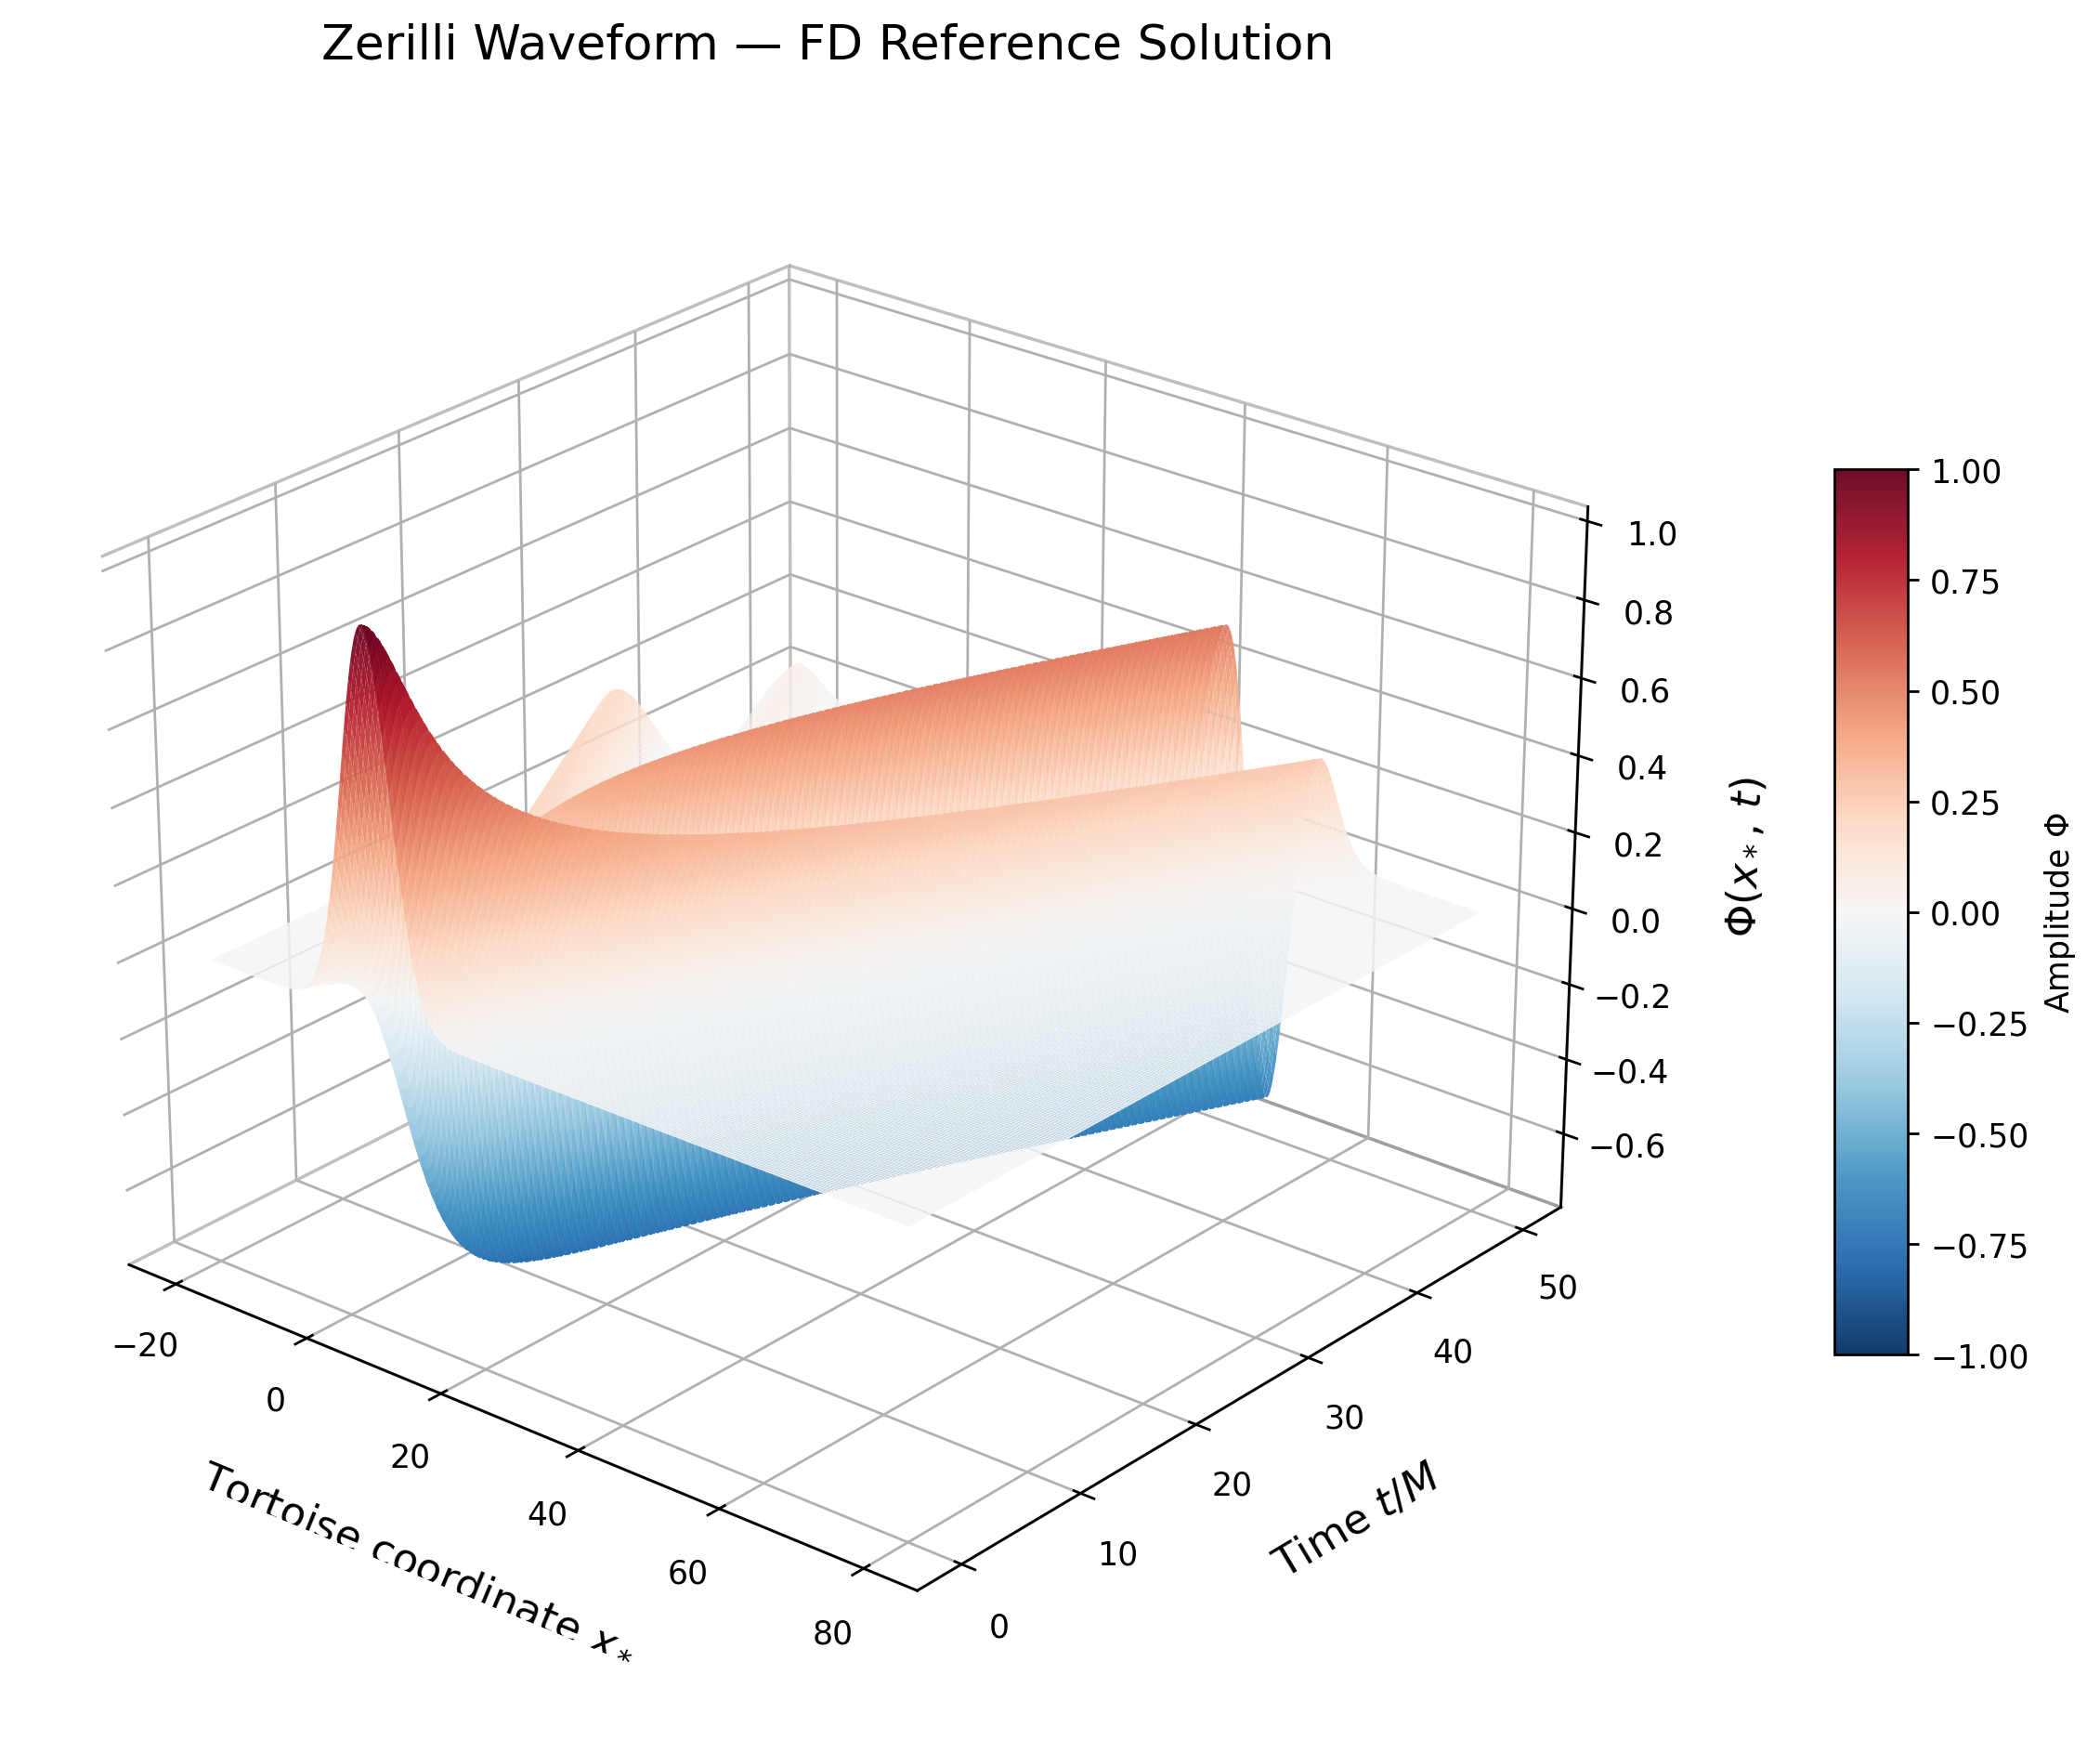
\includegraphics[width=\linewidth]{../outputs/pinn/waveform_3d_zoom.png}
  \subcaption{Zoom around the observer region $x \in [-20,80]\,M$. The
  ringdown is visible as the small-amplitude decaying oscillation
  near $x \simeq 10\,M$ for $t \gtrsim 10\,M$, lying between
  the right-moving free pulse and the back-scattered left-mover.}
  \label{fig:waveform-3d-zoom}
\end{minipage}
\caption{FD reference field $\Phi_{\mathrm{FD}}(x,t)$ for the
Schwarzschild $\ell=2$ Zerilli problem, generated by the fourth-order
Runge--Kutta method-of-lines integration of
Eq.~\eqref{eq:zerilli} with the initial data of
Eq.~\eqref{eq:ic} and the Sommerfeld boundaries of
Eq.~\eqref{eq:bc-sommerfeld}. The Zerilli PINN field-accuracy
metrics in Sec.~\ref{sec:results} are computed against this
reference.}
\label{fig:waveform-3d}
\end{figure}

% --------------------------------------------------------------
\subsection{Forward PINN}
\label{sec:fwd-pinn}

We implement the forward PINN \citep{Raissi2017} in DeepXDE
\citep{Lu2021deepxde} with the PyTorch backend
\citep{Paszke2019pytorch}. Following \citet{Patel2024pinn}, it uses a
fully connected $[80,40,20,10]$ $\tanh$ network with Glorot-uniform
initialisation, coordinates scaled linearly to $[-1,1]^2$, and the
bounded output $\Phi_\theta=A_0\tanh\hat y$. The architecture is held
fixed between the reproduction and enhanced runs, so their comparison
isolates the training schedule, collocation sampling and extraction
protocol. The network has $4{,}521$ trainable parameters.

At each coordinate pair $(x,t)$, the network returns the field value
$\Phi_\theta(x,t)$. Automatic differentiation supplies the derivatives
used to evaluate the Zerilli, initial-data and boundary residuals.
Consequently, no FD field values enter the PINN loss; the FD solution
is retained only for evaluation.

\begin{figure}[!htbp]
\centering
\resizebox{\textwidth}{!}{%
\begin{tikzpicture}[
  node distance=10mm and 12mm,
  every node/.style={font=\small},
  inp/.style={circle, draw, fill=blue!10, minimum size=7mm, inner sep=0pt},
  hid/.style={circle, draw, fill=gray!12, minimum size=4mm, inner sep=0pt},
  outn/.style={circle, draw, fill=orange!20, minimum size=7mm, inner sep=0pt},
  loss/.style={rectangle, draw, fill=green!10, rounded corners=2pt,
               minimum height=6mm, minimum width=18mm, inner sep=2pt,
               align=center, font=\footnotesize},
  arr/.style={->, >=stealth, thin, gray!70},
]
  % Inputs
  \node[inp] (x) at (0, 0) {$x$};
  \node[inp] (t) at (0, -1.2) {$t$};

  % Layer geometry: visually decreasing column heights to reflect 80, 40, 20, 10.
  % Layer 1: 8 nodes, Layer 2: 4 nodes, Layer 3: 2 nodes, Layer 4: 1 node.
  % Use vertical spacing 0.45 cm between nodes; centre each column at y=-0.6.
  \def\xL{2.0}
  \def\xLii{4.0}
  \def\xLiii{6.0}
  \def\xLiv{8.0}

  % Layer 1: 8 nodes, ys from +1.6 to -2.8 (step 0.55)
  \foreach \k/\y in {1/1.6, 2/1.05, 3/0.5, 4/-0.05, 5/-0.6, 6/-1.15, 7/-1.7, 8/-2.25}{
    \node[hid] (a\k) at (\xL, \y) {};
  }
  % Layer 2: 4 nodes, centred at y=-0.6, spacing 0.65
  \foreach \k/\y in {1/0.4, 2/-0.25, 3/-0.9, 4/-1.55}{
    \node[hid] (b\k) at (\xLii, \y) {};
  }
  % Layer 3: 2 nodes
  \foreach \k/\y in {1/-0.2, 2/-1.0}{
    \node[hid] (c\k) at (\xLiii, \y) {};
  }
  % Layer 4: 1 node
  \node[hid] (d1) at (\xLiv, -0.6) {};

  % Layer width labels
  \node[font=\scriptsize] at (\xL, 2.15) {$80$};
  \node[font=\scriptsize] at (\xLii, 0.95) {$40$};
  \node[font=\scriptsize] at (\xLiii, 0.35) {$20$};
  \node[font=\scriptsize] at (\xLiv, -0.05) {$10$};

  % Output
  \node[outn] (phi) at (10.0, -0.6) {$\Phi_\theta$};

  % Connections: fully connected between adjacent shown columns,
  % so every node carries at least one edge (dense-net appearance).
  \foreach \src in {x, t}
    \foreach \dst in {a1,a2,a3,a4,a5,a6,a7,a8}
      \draw[arr, opacity=0.45] (\src) -- (\dst);
  \foreach \a in {1,2,3,4,5,6,7,8}
    \foreach \b in {1,2,3,4}
      \draw[arr, opacity=0.16] (a\a) -- (b\b);
  \foreach \a in {1,2,3,4}
    \foreach \b in {1,2}
      \draw[arr, opacity=0.30] (b\a) -- (c\b);
  \foreach \a in {1,2}
      \draw[arr, opacity=0.45] (c\a) -- (d1);
  \draw[arr] (d1) -- (phi);

  % Loss boxes on the right
  \node[loss, right=14mm of phi, yshift=14mm] (lpde)
    {gPINN: $\mathcal{L}_{\mathrm{r}},\,\mathcal{L}_{\partial_x r},\,\mathcal{L}_{\partial_t r}$};
  \node[loss, right=14mm of phi] (lic)
    {IC: $\mathcal{L}_{\Phi}^{\mathrm{IC}},\,\mathcal{L}_{\partial_t\Phi}^{\mathrm{IC}}$};
  \node[loss, right=14mm of phi, yshift=-14mm] (lbc)
    {BC: $\mathcal{L}_{\mathrm{BC}}^{\mathrm{left}},\,\mathcal{L}_{\mathrm{BC}}^{\mathrm{right}}$};
  \draw[arr, thick, black] (phi) -- (lpde) node[midway, above, font=\scriptsize, sloped] {AD};
  \draw[arr, thick, black] (phi) -- (lic);
  \draw[arr, thick, black] (phi) -- (lbc);

  % Sum to total loss
  \node[loss, fill=green!25, right=8mm of lic] (ltot)
    {$\mathcal{L}_{\mathrm{fwd}}$\\Eq.~\eqref{eq:loss-fwd}};
  \draw[arr, thick, black] (lpde) -| (ltot);
  \draw[arr, thick, black] (lic) -- (ltot);
  \draw[arr, thick, black] (lbc) -| (ltot);

  % Section labels (placed above the layer columns).
  \node[font=\scriptsize, gray!70!black] at (0.0, 2.7) {inputs};
  \node[font=\scriptsize, gray!70!black] at (5.0, 2.7) {$[80,40,20,10]$ tanh MLP};
  \node[font=\scriptsize, gray!70!black] at (10.0, 2.7) {output transform};
  \node[font=\scriptsize, gray!70!black] at (13.5, 2.7) {weighted loss terms};
\end{tikzpicture}}
\caption{Forward PINN architecture used in this work. The physical
inputs $(x,t)$ are linearly normalised and passed through a fully
connected $[80,40,20,10]$ $\tanh$ network with $4{,}521$ trainable
parameters, whose scalar output is wrapped in the tanh envelope
$\Phi_\theta(x,t) = A\tanh(\hat y(x,t))$ with $A = 1$. Spatial and
temporal derivatives required by the Zerilli PDE residual
$\mathcal{L}_{\mathrm{r}}$ of Eq.~\eqref{eq:loss-fwd} and its
gradient augmentations $\mathcal{L}_{\partial_x r},
\mathcal{L}_{\partial_t r}$ (gPINN, \citealt{Yu2022gpinn}) are
computed by automatic differentiation; the IC residuals
$\mathcal{L}_{\Phi}^{\mathrm{IC}}, \mathcal{L}_{\partial_t\Phi}^{\mathrm{IC}}$ and the left/right BC residuals
$\mathcal{L}_{\mathrm{BC}}^{\mathrm{left}}, \mathcal{L}_{\mathrm{BC}}^{\mathrm{right}}$ enter as additional weighted terms with
$\boldsymbol{\lambda} = (100,100,100,1,100,1,1)$
(Eq.~\eqref{eq:weights}).}
\label{fig:fwd-pinn-arch}
\end{figure}

Let $r_\theta(x,t) \equiv \partial_t^2\Phi_\theta -
\partial_x^2\Phi_\theta + V_\ell\,\Phi_\theta$ be the pointwise
residual of Eq.~\eqref{eq:zerilli}, with
$V_\ell=V_\ell^{\mathrm{Z}}$ for the Zerilli runs. The loss is the
weighted mean-squared sum of the PDE, initial-data and boundary
residuals, augmented by the two gradient-enhanced PINN terms
\citep{Yu2022gpinn},
\begin{equation}
  \mathcal{L}_{\mathrm{fwd}}
  = \lambda_{r}     \Lpde
  + \lambda_{r_x}   \mathcal{L}_{\partial_x r}
  + \lambda_{r_t}   \mathcal{L}_{\partial_t r}
  + \lambda_{\mathrm{IC}} \mathcal{L}_{\Phi}^{\mathrm{IC}}
  + \lambda_{\mathrm{IV}} \mathcal{L}_{\partial_t\Phi}^{\mathrm{IC}}
  + \lambda_{\mathrm{BL}} \mathcal{L}_{\mathrm{BC}}^{\mathrm{left}}
  + \lambda_{\mathrm{BR}} \mathcal{L}_{\mathrm{BC}}^{\mathrm{right}}.
  \label{eq:loss-fwd}
\end{equation}
The seven mean-squared component losses are
\begin{align}
  \Lpde &= \frac{1}{N_r}\sum_{(x,t)\in\mathcal{X}_r}
            r_\theta(x,t)^{2},
  & \mathcal{L}_{\partial_x r} &= \frac{1}{N_r}\sum_{(x,t)\in\mathcal{X}_r}
            \bigl(\partial_x r_\theta(x,t)\bigr)^{2},
  \nonumber\\
  \mathcal{L}_{\partial_t r} &= \frac{1}{N_r}\sum_{(x,t)\in\mathcal{X}_r}
            \bigl(\partial_t r_\theta(x,t)\bigr)^{2},
  & \mathcal{L}_{\Phi}^{\mathrm{IC}} &= \frac{1}{N_i}\sum_{x\in\mathcal{X}_i}
            \bigl(\Phi_\theta(x,0)-\Phi(x,0)\bigr)^{2},
  \nonumber\\
  \mathcal{L}_{\partial_t\Phi}^{\mathrm{IC}}
     &= \frac{1}{N_i}\sum_{x\in\mathcal{X}_i}
        \bigl(\partial_t\Phi_\theta(x,0)-\partial_t\Phi(x,0)\bigr)^{2},
  & \mathcal{L}_{\mathrm{BC}}^{\mathrm{left}}
     &= \frac{1}{N_b}\sum_{t\in\mathcal{X}_b^{L}}
        \bigl((\partial_t-\partial_x)\Phi_\theta(x_{\min},t)\bigr)^{2},
  \nonumber\\
  \mathcal{L}_{\mathrm{BC}}^{\mathrm{right}}
     &= \frac{1}{N_b}\sum_{t\in\mathcal{X}_b^{R}}
        \bigl((\partial_t+\partial_x)\Phi_\theta(x_{\max},t)\bigr)^{2},
  & &
  \label{eq:loss-components}
\end{align}
These terms follow \citet[Eqs.~(4)--(10)]{Patel2024pinn}. We use
$N_r=32{,}000$, $N_i=800$ and $N_b=400$ total boundary points.
\citet{Patel2024pinn} describe $400$ points per boundary, which is the
only collocation-count difference in the reproduction. The two
gradient terms penalise spatial and temporal variation of the PDE
residual, following \citet{Yu2022gpinn}. The
forward-PINN weight vector is
\begin{equation}
  \boldsymbol{\lambda}
  = (\lambda_{r},\lambda_{r_x},\lambda_{r_t},\lambda_{\mathrm{IC}},
     \lambda_{\mathrm{IV}},\lambda_{\mathrm{BL}},\lambda_{\mathrm{BR}})
  = (100,\,100,\,100,\,1,\,100,\,1,\,1),
  \label{eq:weights}
\end{equation}
following \citet{Patel2024pinn}. The larger
$\lambda_{\mathrm{IV}}=100$ weights the initial-velocity residual,
which Patel et al. identify as important for controlling phase drift.
The unit Sommerfeld weights are consistent with the causal remoteness
of the finite boundaries in Eq.~\eqref{eq:bc-arrival}.

The reproduction run uses the optimiser schedule of
\citet{Patel2024pinn}, namely Adam \citep{Kingma2015adam} for
$10^4$ iterations followed by L-BFGS \citep{Liu1989lbfgs} for
$1.5\times10^4$ iterations. The enhanced forward PINN keeps Adam
fixed and doubles the L-BFGS budget to $3\times10^4$ iterations
(Table~\ref{tab:train-config}), since the loss continues to decrease
through iteration $\sim 25{,}000$. All PINN training is full-batch
and uses double precision; in single precision the L-BFGS phase
stalled in our runs. During the Adam phase of the enhanced run, every
$1{,}000$ optimiser iterations the greedy resampler
\citep{Lu2021deepxde,Wu2023adaptive} scores $10^5$ uniformly drawn
candidates by the primary PDE residual $|r_\theta|$ and replaces the
interior collocation set with $0.3N_r$ highest-residual points and
$0.7N_r$ uniformly drawn points. The uniform component preserves
coverage away from the wavefront.

% --------------------------------------------------------------
\subsection{The Schwarzschild hFNO}
\label{sec:hyb-method}

Unlike the per-instance PINN, the hFNO is trained on the sampled
$(M,x_0,\sigma)$ configurations to approximate the
discretisation-error correction for each configuration. For a
parameter triple
$q=(M,x_0,\sigma)$, let $\Phi_k^{\mathrm c}(q)$ denote the full FD
field computed with grid factor $k$, and define the upsampled
deployment prior $P(q)=\mathcal U\Phi_4^{\mathrm c}(q)$. The
corresponding map is
\begin{equation}
  \mathcal G_\theta^{\mathrm{hyb}}(q)
  =P(q)+g[P(q)]\,\mathcal H_\theta(X(q)),
  \label{eq:hyb-map}
\end{equation}
where $\mathcal H_\theta$ returns an additive correction on the
same fine $(t,x)$ grid as $P$.

The FNO does not advance the Zerilli equation in time. The FD solver
computes the coarse-grid finite-difference solution on the full
$(t,x)$ domain before the FNO returns its correction in a single
forward pass. This differs from
recurrent solver-in-the-loop training, which modifies each numerical
step \citep{Um2020solverloop,Kochkov2021mlcfd}. The FD fields are
precomputed and no gradients pass through the solver.

During training, for each parameter triple, the corresponding $k=4$
and $k=2$ fields form a Richardson-extrapolated field. The
gated FNO output is fitted to the difference between that estimate
and $P$. The fine FD reference field
does not enter the optimisation objective and is used only to evaluate
the reconstructed field. At inference, the $k=2$ solve, Richardson
construction and fine reference field are absent. A new configuration requires
one $k=4$ solve, quintic upsampling and one FNO evaluation.
The training tensors and canonical evaluation use quintic
interpolation. The archived $100$-configuration population evaluation
uses the legacy cubic interpolation path; its reported field and QNM
statistics therefore refer to that evaluation path.

The coordinate grid, $x_0$, $\sigma$ and $\xq$ are fixed code
coordinates while $M$ varies. Only the canonical $M=1$ configuration
identifies these numerical coordinate values directly with units of
$M$.

\begin{table}[!htbp]
\centering
\caption{Schwarzschild hFNO architecture, parameter domain and
dataset.}
\label{tab:surrogate-config}
\footnotesize
\setlength{\tabcolsep}{5pt}
\begin{tabular}{@{}lc@{}}
\toprule
 & Schwarzschild hFNO \\
\midrule
Domain $x\times t$ (code coordinates) & $[-50,150]\times[0,100]$ \\
Grid $N_{x}\times N_{t}$ (fine) & $1001\times 1001$ \\
Coarse grids & $k{=}4$ prior; $k{=}2,4$ Richardson pair \\
Input channels & $5$ \\
Hidden channels $h$ & $32$ \\
Fourier modes $(K_{t},K_{x})$ & $(16,32)$ \\
Domain padding & $0.10$ \\
Parameters & $1.13\times 10^{6}$ \\
$M$ & $\mathrm{Unif}[0.8,1.2]$ \\
$x_{0}$ & $\mathrm{Unif}[2,6]$ \\
$\sigma$ & $\mathrm{Unif}[3,7]$ \\
Samples (Sobol seed $0$) & $1000/100/100$ \\
Training seed & $1234$ \\
Loss & Eq.~\eqref{eq:hyb-loss} \\
Observer $\xq$ (code coordinate) & $10$ \\
Canonical $(M,x_{0},\sigma)$ & $(1,4,5)$ \\
\bottomrule
\end{tabular}
\end{table}

\begin{figure}[!htbp]
\centering
\resizebox{0.78\textwidth}{!}{%
\begin{tikzpicture}[
  every node/.style={font=\small},
  ic/.style={rectangle, draw, fill=yellow!18, rounded corners=2pt,
             minimum height=8mm, minimum width=42mm, inner sep=3pt,
             align=center},
  fd/.style={rectangle, draw, fill=red!12, rounded corners=2pt,
             minimum height=11mm, minimum width=58mm, inner sep=3pt,
             align=center},
  up/.style={rectangle, draw, fill=red!6, rounded corners=2pt,
             minimum height=10mm, minimum width=58mm, inner sep=3pt,
             align=center},
  inp/.style={rectangle, draw, fill=blue!10, rounded corners=2pt,
              minimum height=7mm, minimum width=88mm, inner sep=3pt,
              align=center, font=\small},
  stack/.style={rectangle, draw=none, fill=none,
                inner sep=2pt, align=center, font=\small},
  stackbg/.style={rectangle, draw, fill=blue!5, rounded corners=3pt,
                  inner sep=4pt},
  fnobox/.style={rectangle, draw, fill=gray!12, rounded corners=2pt,
                 minimum height=14mm, minimum width=58mm, inner sep=3pt,
                 align=center},
  fnoblock/.style={rectangle, draw=none, fill=none,
                   inner sep=2pt, align=center},
  fnobg/.style={rectangle, draw, fill=gray!18, rounded corners=3pt,
                inner sep=5pt},
  outn/.style={rectangle, draw, fill=orange!25, rounded corners=2pt,
               minimum height=10mm, minimum width=58mm, inner sep=3pt,
               align=center},
  sum/.style={circle, draw, fill=green!20, inner sep=0pt,
              minimum size=9mm, font=\large},
  loss/.style={rectangle, draw, fill=green!12, rounded corners=2pt,
               minimum height=10mm, minimum width=68mm, inner sep=3pt,
               align=center},
  arr/.style={->, >=stealth, thick, black},
  arrs/.style={->, >=stealth, thick, blue!55!black, dashed},
  arrt/.style={->, >=stealth, thick, gray!55!black, dashed},
  sec/.style={font=\footnotesize\itshape, gray!55!black, anchor=west},
]
  % ============ classical solver path ============
  \node[ic]   (icbox) {initial data $(M,\,x_{0},\,\sigma)$};
  \node[fd, below=4mm of icbox]
        (cfd)   {coarse RK4 method-of-lines, 2nd-order stencil\\
                 $(\Delta x,\Delta t)_{\mathrm{c}}=(0.8,0.4)\,M$ \\
           grid $251\times 251$ ($k=4$)};
  \node[up, below=4mm of cfd]
        (upbox) {quintic-spline upsample $\mathcal{U}$ in $(t,x)$\\
           (Eq.~\eqref{eq:hyb-upsample}, fine grid $1001\times 1001$)};

  \draw[arr] (icbox) -- (cfd);
  \draw[arr] (cfd) -- (upbox);

  % ============ five-channel input stack ============
  \node[stack, below=6mm of upbox] (stackhdr) {%
    \textbf{five-channel input on fine grid}\;
    $X\in\mathbb{R}^{5\times N_{t}\times N_{x}}$};
  \node[inp, below=2mm of stackhdr]
      (c0) {ch~0: $\mathcal{U}\Phi^{\mathrm{c}}(x,t)$, quintic-upsampled $k{=}4$ prior};
  \node[inp, below=1mm of c0]
        (c1) {ch~1: $\Phi^{\mathrm{c}}(x,0)$ broadcast in $t$};
  \node[inp, below=1mm of c1]
        (c2) {ch~2: $V_{\ell}(x;M)$ broadcast in $t$};
  \node[inp, below=1mm of c2]
        (c3) {ch~3: $M$ broadcast over $(x,t)$};
  \node[inp, below=1mm of c3]
        (c4) {ch~4: $\Pi^{\mathrm{c}}_{0}(x)$ broadcast in $t$
              (Eq.~\eqref{eq:hyb-pi0})};
  \begin{scope}[on background layer]
    \node[stackbg, fit=(stackhdr)(c0)(c4)] (stackbg) {};
  \end{scope}

  \draw[arr] (upbox) -- (stackbg.north);

  % ============ FNO correction operator ============
  \node[fnoblock, below=8mm of stackbg.south] (fnohdr) {%
    \begin{minipage}{96mm}
      \centering
      \textbf{neural correction operator $\mathcal{H}_{\theta}$, four-layer 2-D FNO}\\[1mm]
      hidden channels $h=32$,\;
      Fourier modes $(K_{t},K_{x})=(16,32)$,\;
      domain padding $0.10$
    \end{minipage}};

  \node[fnobox, below=3mm of fnohdr]
        (lift)  {lift $1{\times}1$ conv: $5{\to}32$ channels};
  \node[fnobox, below=2mm of lift]
        (sb)    {$L=4 \times$ spectral block\\
                 $v^{(\ell+1)}=\mathrm{GELU}\bigl(
                  \mathcal{F}^{-1}[R^{(\ell)}{\odot}\mathcal{F}v^{(\ell)}]
                  + W^{(\ell)}v^{(\ell)}\bigr)$};
  \node[fnobox, below=2mm of sb]
        (proj)  {projection $1{\times}1$ conv: $32{\to}1$ channel};

  \draw[arr] (lift) -- (sb);
  \draw[arr] (sb) -- (proj);
  \begin{scope}[on background layer]
    \node[fnobg, fit=(fnohdr)(lift)(proj)] (fnoall) {};
  \end{scope}

  \draw[arr] (stackbg.south) -- (fnoall.north);

    % ============ output correction + reconstruction ============
  \node[outn, below=8mm of fnoall.south]
      (delta) {$g\,\delta\Phi_{\theta}(x,t)$, gated correction\\
           $g=d_{\mathrm{idx}}/(d_{\mathrm{idx}}+s),\;s{=}10^{-3}$\\
                 (Eq.~\eqref{eq:hyb-gate})};
  \draw[arr] (fnoall.south) -- (delta.north);

  % sum node and Phi_hybrid
  \node[sum, below=8mm of delta] (sumn) {$+$};
  \node[outn, fill=orange!45, below=4mm of sumn]
        (phih)  {$\Phi^{\mathrm{hyb}}(x,t)
                 =\mathcal{U}\Phi^{\mathrm{c}}+g\,\delta\Phi_{\theta}$\\
                 (Eq.~\eqref{eq:hyb-reconstruct})};
  \draw[arr] (delta) -- (sumn);
  \draw[arr] (sumn) -- (phih);

  % skip connection from upsample (long curve down the left)
  \draw[arrs] (upbox.west) -- ++(-3.6,0) |-
              node[pos=0.10, anchor=south, rotate=90, font=\scriptsize, blue!55!black, yshift=2pt]
                      {numerical prior: $\mathcal{U}\Phi^{\mathrm{c}}$}
              (sumn.west);

  % training-only target + loss (right side, dashed)
  \node[outn, fill=red!18, right=22mm of delta]
        (target){Richardson correction target from coarse solves\\
                 $\delta\Phi_{\mathrm{R}}=\Phi^{\mathrm{R}}-\mathcal{U}\Phi^{\mathrm{c}}$\\
                 (Eqs.~\eqref{eq:hyb-richardson},\eqref{eq:hyb-residual})};
  \node[loss, below=4mm of target]
        (lhyb)  {$\mathcal{L}_{\mathrm{hyb}}
                 =\mathrm{MSE}\bigl(g\,\delta\Phi_{\theta},\,\delta\Phi_{\mathrm{R}}\bigr)$\\
                 (Eq.~\eqref{eq:hyb-loss})};
  \draw[arrt] (delta.east) --
              node[pos=0.60, above, font=\scriptsize, gray!55!black] {training only}
              (target.west);
  \draw[arr]  (target) -- (lhyb);

  % gradient backflow from loss to FNO (training only)
  \draw[arrt, gray!65!black] (lhyb.east) -- ++(0.5,0) |-
              node[pos=0.25, anchor=south, rotate=90, font=\scriptsize, gray!55!black, yshift=2pt]
            {$\nabla_{\theta}\mathcal{L}_{\mathrm{hyb}}$}
              (fnoall.east);
\end{tikzpicture}
}
\caption{Schwarzschild hFNO pipeline of Sec.~\ref{sec:hyb-method}.
The classical RK4
method-of-lines solver of Appendix~\ref{app:fd} produces the
coarse field $\Phi^{\mathrm{c}}$ on
$(\Delta x,\Delta t)_{\mathrm{c}} = (0.8,0.4)\,M$ ($k=4$), which
is quintic-spline upsampled in $(t,x)$ onto the fine grid by the
operator $\mathcal{U}$ of Eq.~\eqref{eq:hyb-upsample}. The
five-channel input stack combines this prior
$\mathcal{U}\Phi^{\mathrm{c}}$ with the initial displacement
$\Phi^{\mathrm{c}}(x,0)$, initial velocity
$\Pi^{\mathrm{c}}_{0}(x)$ (Eq.~\eqref{eq:hyb-pi0}), Zerilli
potential $V_{\ell}(x;M)$ and broadcast mass $M$. A four-layer
2-D FNO $\mathcal{H}_{\theta}$ with hidden channel count
$h = 32$ and retained Fourier modes $(K_{t},K_{x}) = (16,32)$
predicts an additive correction, which is multiplied by the
deterministic fixed-scale gradient gate
$g=d_{\mathrm{idx}}/(d_{\mathrm{idx}}+s)$
(Eq.~\eqref{eq:hyb-gate}, $s = 10^{-3}$, a deterministic
function of the prior) before being added back; the hybrid
prediction Eq.~\eqref{eq:hyb-reconstruct} adds the
quintic-upsampled coarse field explicitly (blue dashed),
and the gate confines the correction to the under-resolved
wavefronts. The dashed grey path on the right depicts the
training-only Richardson correction target
$\delta\Phi_{\mathrm{R}} = \Phi^{\mathrm{R}} -
\mathcal{U}\Phi^{\mathrm{c}}$
(Eqs.~\eqref{eq:hyb-richardson},\eqref{eq:hyb-residual}), built
from $k = 4$ and $k = 2$ coarse solves alone, and the MSE loss
Eq.~\eqref{eq:hyb-loss} against which $\mathcal{H}_{\theta}$ is
fitted; at inference time the right-hand path is absent and
only the single $k = 4$ coarse solve and the left-hand
reconstruction path are evaluated. Total trainable parameters:
$1.13\times 10^{6}$.}
\label{fig:hyb-arch}
\end{figure}

\paragraph{Discretisation and grids.} The fine and coarse solves use
the same physical domain and the same RK4 method-of-lines scheme as
Appendix~\ref{app:fd}, with the same second-order centred stencil.
The fine evolution has $N_x=1001$ points and $N_{\mathrm{step}}=1000$
time steps, while the $k=4$ prior has $N_x=251$ and
$N_{\mathrm{step}}=250$. Since every RK4 stage is linear in $N_x$,
the coarse-to-fine ratio of finite-difference point updates is
\begin{equation}
  \frac{N_x^{\mathrm c}N_{\mathrm{step}}^{\mathrm c}}
       {N_x^{\mathrm f}N_{\mathrm{step}}^{\mathrm f}}
  = \frac{251\times250}{1001\times1000}
  \approx \frac{1}{16}.
  \label{eq:hyb-work-ratio}
\end{equation}

\paragraph{Richardson-extrapolated field and correction target.} For the second-order
stencil, the leading coarse-grid error is
$\mathcal{O}(\Delta x_{\mathrm{c}}^2)$. We upsample the $k=4$ and
$k=2$ fields with $\mathcal{U}$ and form the Richardson-extrapolated field in
Eq.~\eqref{eq:hyb-richardson}.
\begin{equation}
  \Phi^{\mathrm{R}}
  \;=\; \frac{4\,\mathcal{U}\Phi^{\mathrm{c}}_{2}
              - \mathcal{U}\Phi^{\mathrm{c}}}{3},
  \label{eq:hyb-richardson}
\end{equation}
This cancels the leading error, giving
$\Phi^{\mathrm{R}}=\Phi+\mathcal{O}(\Delta x_{\mathrm{c}}^4)$ up to
interpolation error. The correction target is
\begin{equation}
  \delta\Phi_{\mathrm{R}}(x, t)
  \;=\; \Phi^{\mathrm{R}}(x, t) - \mathcal{U}\Phi^{\mathrm{c}}(x, t),
  \label{eq:hyb-residual}
\end{equation}
and agrees with the true coarse-grid error up to the remaining
fourth-order Richardson and interpolation errors. It is obtained
entirely from coarse solves. The fine reference field is used only for
evaluation, while inference requires only the $k=4$ solve. The target
is concentrated on under-resolved wavefronts, motivating the gate in
Eq.~\eqref{eq:hyb-gate}.

\paragraph{Upsample operator.} The operator $\mathcal{U}$ is the
degree-five tensor-product spline
\begin{equation}
  (\mathcal{U}\Phi^{\mathrm{c}})(x, t)
  \;=\; \sum_{i, j} c_{ij}\,
        B_{5}\!\Bigl(\tfrac{t - t_{i}}{\Delta t_{\mathrm{c}}}\Bigr)\,
        B_{5}\!\Bigl(\tfrac{x - x_{j}}{\Delta x_{\mathrm{c}}}\Bigr),
  \label{eq:hyb-upsample}
\end{equation}
Here $B_5$ is the quintic B-spline basis and the coefficients
interpolate the coarse nodes. The same operator is applied to both
coarse fields. For smooth data, its formal order exceeds the
fourth-order Richardson remainder, and its interpolation error is
smaller than the correction target in the tested regime.

\paragraph{Input stack.} The input contains the upsampled prior,
initial displacement, Zerilli potential, broadcast mass and the
initial velocity estimate
\begin{equation}
  \Pi^{\mathrm{c}}_{0}(x)
  \;=\; \frac{\Phi^{\mathrm{c}}(x, \Delta t_{\mathrm{c}}) -
              \Phi^{\mathrm{c}}(x, 0)}{\Delta t_{\mathrm{c}}},
  \label{eq:hyb-pi0}
\end{equation}
computed on the coarse grid and linearly resampled to the fine $x$
grid. The velocity is an auxiliary input rather than a supervised
target. The prior channel supplies the coarse evolution.
The parameters $x_0$ and $\sigma$ are encoded by the initial
displacement and velocity fields, while $M$ is supplied explicitly
and through the potential. Thus $X$ identifies both the initial-value
problem and the spatial operator whose discretisation error is being
corrected.

\paragraph{Correction operator, gradient gate, and reconstruction.}
The neural correction operator
\begin{equation}
  \mathcal{H}_{\theta}\colon\;
  X = \bigl[\mathcal{U}\Phi^{\mathrm{c}},\,\Phi^{\mathrm{c}}(\cdot, 0),\,
            V_{\ell}(\cdot; M),\,M,\,\Pi^{\mathrm{c}}_{0}\bigr]
  \;\longmapsto\;
  \delta\Phi_{\theta}(x, t)
  \label{eq:hyb-operator}
\end{equation}
is modulated by a deterministic fixed-scale gradient gate before it is
added to the prior. For $P_{ij}=P(x_j,t_i)$, the implementation forms
the index-space gradient magnitude
\begin{equation}
  d_{\mathrm{idx},ij}
  = \sqrt{(\Delta_i P_{ij})^2+(\Delta_j P_{ij})^2},
  \qquad
  g_{ij}=\frac{d_{\mathrm{idx},ij}}{d_{\mathrm{idx},ij}+s},
  \label{eq:hyb-gate}
\end{equation}
where $\Delta_i$ and $\Delta_j$ are the finite differences returned
with unit grid-index spacing. On the fixed $1001\times1001$ grid, we
set $s=Q_{0.68}(d_{\mathrm{idx}})=10^{-3}$ using only the deployment
prior. The gate is a deterministic function of the prior alone. It
approaches one on wavefronts with large
$d_{\mathrm{idx}}$, where the numerical prior has its largest
dispersion error, and
zero in smooth regions away
from the wavefronts, including the numerically zero region ahead of
the outgoing signal. The corrected field is reconstructed by adding
the gated FNO correction to the interpolated coarse solution,
\begin{equation}
  \Phi^{\mathrm{hyb}}(x, t)
  \;=\; \mathcal{U}\Phi^{\mathrm{c}}(x, t)
         + g(x, t)\,\mathcal{H}_{\theta}(X)(x, t),
  \label{eq:hyb-reconstruct}
\end{equation}
which confines the correction to the under-resolved regions by
construction and reduces to the quintic-upsampled coarse solve
(the upsampled numerical prior of Sec.~\ref{sec:res-hyb}) wherever
$g = 0$ or $\mathcal{H}_{\theta} \equiv 0$.

\paragraph{FNO architecture.} The correction operator
$\mathcal{H}_{\theta}$ is a 2-D Fourier neural operator
\citep{Li2021fno,Kovachki2023neuralop} on the fine $(t, x)$
grid: a $1\times 1$ lift to $h = 32$ hidden channels, $L = 4$
Fourier layers of the form
\begin{equation}
  v^{(\ell+1)}(x, t)
  \;=\; \mathrm{GELU}\!\Bigl(
         \mathcal{F}^{-1}\bigl[R^{(\ell)} \odot
         \mathcal{F}\,v^{(\ell)}\bigr](x, t)
         \;+\; W^{(\ell)}\,v^{(\ell)}(x, t)
       \Bigr),
  \label{eq:hyb-fno-layer}
\end{equation}
and a $1\times 1$ projection back to one channel, where
$\mathcal{F}$ is the 2-D DFT along $(t, x)$, $R^{(\ell)}$ the
complex spectral-weight tensor truncated to
$(K_{t}, K_{x}) = (16, 32)$ retained modes (matching the $2{:}1$
spatial-to-temporal domain-length ratio and resolving
$k_{x} \lesssim 1.0\,M^{-1}$), $\odot$ mode-by-mode matrix
multiplication across channels, and $W^{(\ell)}$ a pointwise
linear path. Each axis is pre-padded by $p = 0.10$ against
periodic wraparound, and positional $(x, t)$ encodings break
translation equivariance to distinguish the source region from
the wave zones. The total parameter count is $1.13\times 10^{6}$ under the
\texttt{neuraloperator} implementation \citep{Kovachki2023neuralop}.
The lift first maps the five physical inputs to $h$ feature fields.
Within each layer, the Fourier path couples retained modes and feature
channels globally over the complete space-time domain, while
$W^{(\ell)}$ supplies a local pointwise update. The inverse transform
returns the global update to physical space, GELU combines the two
paths nonlinearly, and the final projection returns one correction
field. The smaller width is used because the FNO predicts a
correction rather than the full field.

\paragraph{Loss.} The training loss is the gridwise mean
squared error between the gated network output and the
Richardson correction target built from coarse solves,
\begin{equation}
  \mathcal{L}_{\mathrm{hyb}}(\theta)
  \;=\; \frac{1}{B}\sum_{b=1}^{B}
         \frac{1}{N_{t} N_{x}}
         \sum_{i=1}^{N_{t}}\sum_{j=1}^{N_{x}}
         \bigl[
           g^{(b)}_{ij}\,\mathcal{H}_{\theta}(X^{(b)})_{ij}
           \,-\, \delta\Phi^{(b)}_{\mathrm{R},\,ij}
         \bigr]^{2},
  \label{eq:hyb-loss}
\end{equation}
Because the gate is part of the forward map, the loss trains the
correction after gating rather than the raw FNO output. No auxiliary,
spatially weighted or sample-normalisation terms are used.

\paragraph{Optimiser.} The hFNO is trained with AdamW for $100$ epochs
using the settings in Table~\ref{tab:train-config}. The checkpoint
with the lowest validation MSE is used for evaluation.

\paragraph{Training data.} The Sobol parameter ranges, dataset sizes
and canonical configuration are listed in
Table~\ref{tab:surrogate-config}. The fine, $k = 4$ and $k = 2$
solves are precomputed and cached for the same Sobol triples, so each
Richardson pair represents one initial-value problem. The ranges of
$x_0$ and $\sigma$ keep the prompt burst within the simulation window
for all sampled configurations.

% --------------------------------------------------------------
\subsection{Kerr radial Teukolsky evolution}
\label{sec:teukolsky-numerics}

The Kerr calculation uses a $1+1$ radial model for the $(4,2,0)$ mode
derived from the spin-weight $s=-2$ Teukolsky equation in minimal-gauge
horizon-penetrating hyperboloidal coordinates
\citep{Zenginoglu2011,Harms2013,PanossoMacedo2020}. The compactified
radial coordinate is
\begin{equation}
  \sigma = \frac{r_{+}}{r} \in [0, 1],
  \qquad
  \sigma = 1 \ \text{(horizon)}, \quad
  \sigma = 0 \ (\scri),
  \label{eq:kerr-sigma}
\end{equation}
The time coordinate is replaced by a hyperboloidal time $\tau$ whose
constant-time slices connect the horizon to $\scri$
(Fig.~\ref{fig:kerr-slicing}). On this slice the radial
characteristics leave the domain at both endpoints, into the horizon
and through $\scri$. The evolution is therefore fixed by regular
initial data, with no external boundary data imposed
\citep{Harms2013,PanossoMacedo2020}. To keep the evolved field finite
at both endpoints we use
\begin{equation}
  \Psi = \psi\,\sigma^{3}\,(1 - \sigma)^{-2 - i\beta},
  \qquad
  \beta = \frac{m a}{r_{+} - r_{-}},
  \label{eq:kerr-rescale}
\end{equation}
where $\sigma^3$ accounts for the asymptotic peeling at $\scri$, while
$(1-\sigma)^{-2-i\beta}$ regularises the horizon behaviour. The phase
$\beta = ma/(r_+-r_-)$ carries the spin-dependent azimuthal
frame-dragging contribution.

\begin{figure}[!htbp]
\centering
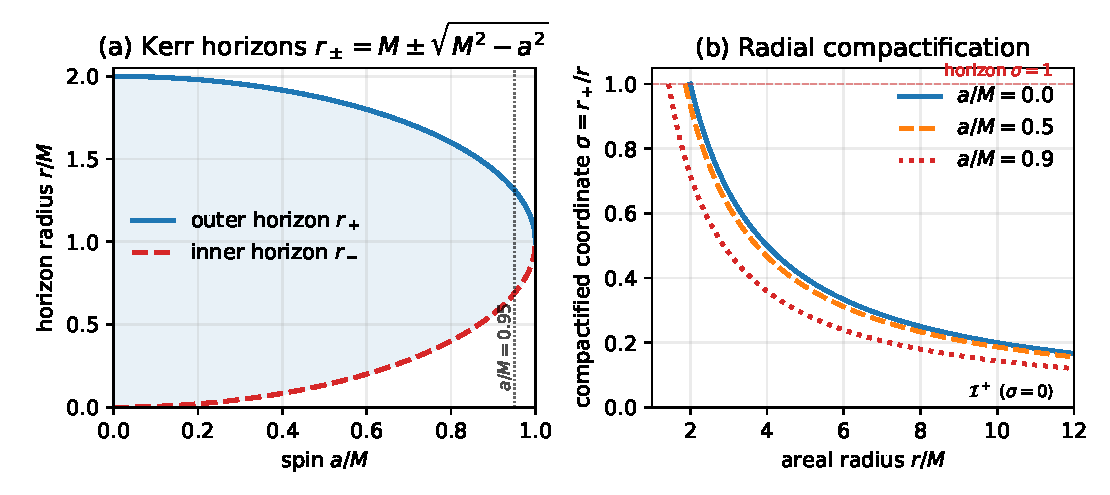
\includegraphics[width=0.92\textwidth]{../outputs/background/kerr_horizons.pdf}
\caption{Kerr geometry and radial coordinate. (a) The outer and
inner horizons $r_{\pm} = M \pm \sqrt{M^{2}-a^{2}}$
(Eq.~\eqref{eq:kerr-horizons}) as functions of spin; they
coincide at extremality $a = M$, and the study range reaches
$a/M = 0.95$ (dotted). (b) The compactification
$\sigma = r_{+}/r$ of Eq.~\eqref{eq:kerr-sigma} for three spins,
mapping the exterior $r \in [r_{+}, \infty)$ onto
$\sigma \in [0, 1]$ with the horizon at $\sigma = 1$ and future
null infinity $\scri$ at $\sigma = 0$. It replaces the finite
tortoise-grid description used for the Schwarzschild calculation.}
\label{fig:kerr-coords}
\end{figure}

\begin{figure}[!htbp]
\centering
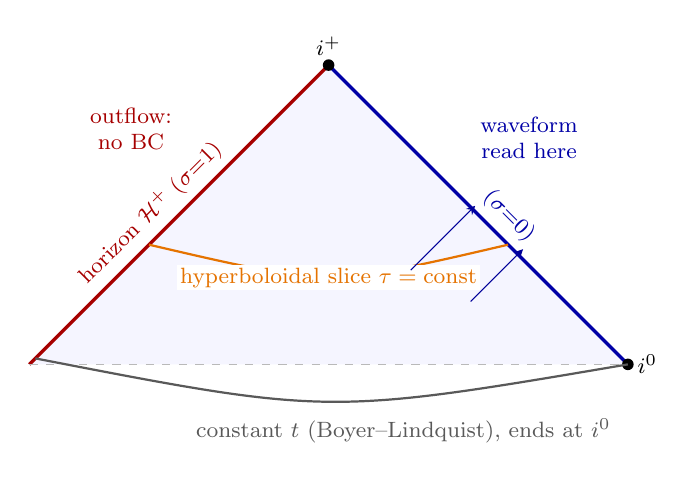
\begin{tikzpicture}[scale=1.9, >=stealth,
                    every node/.style={font=\footnotesize}]
  \coordinate (B)  at (0,0);
  \coordinate (i0) at (4,0);
  \coordinate (ip) at (2,2);
  \fill[blue!4] (B) -- (i0) -- (ip) -- cycle;
  % future horizon (sigma=1) and null infinity (sigma=0)
  \draw[very thick, red!65!black]  (B)  -- (ip);
  \draw[very thick, blue!65!black] (i0) -- (ip);
  \draw[gray!55, dashed] (B) -- (i0);
  \fill (i0) circle (1.1pt);  \fill (ip) circle (1.1pt);
  \node[right]      at (i0) {$i^{0}$};
  \node[above]      at (ip) {$i^{+}$};
  \node[red!65!black, rotate=45, anchor=south, xshift=-3pt]
       at (0.95,0.95) {horizon $\mathcal{H}^{+}\ (\sigma{=}1)$};
  \node[blue!65!black, rotate=-45, anchor=south, xshift=3pt]
       at (3.05,0.95) {$\scri\ (\sigma{=}0)$};
  % Boyer-Lindquist constant-t slice: ends at i^0
  \draw[thick, gray!70!black] (0.04,0.04) .. controls (2,-0.34) .. (i0);
  \node[gray!70!black, below, align=center] at (2.5,-0.30)
       {constant $t$ (Boyer--Lindquist),\ ends at $i^{0}$};
  % hyperboloidal slice: horizon -> scri
  \draw[thick, orange!90!black]
       (0.80,0.80) .. controls (2,0.52) .. (3.20,0.80);
  \node[orange!90!black, fill=white, inner sep=1pt, align=center]
       at (2.0,0.58) {hyperboloidal slice $\tau=\mathrm{const}$};
  % outgoing radiation (slope +1) reaching scri
  \draw[->, blue!60!black] (2.55,0.63) -- (2.98,1.06);
  \draw[->, blue!60!black] (2.95,0.42) -- (3.30,0.77);
  % annotations
  \node[red!65!black,  align=center, anchor=north] at (0.68,1.78)
       {outflow:\\ no BC};
  \node[blue!65!black, align=center, anchor=north] at (3.34,1.72)
       {waveform\\ read here};
\end{tikzpicture}
\caption{Conformal (Penrose) diagram of the Kerr exterior in the
hyperboloidal minimal gauge. The exterior is bounded by the
future horizon $\mathcal{H}^{+}$ ($\sigma = 1$, red) and future
null infinity $\scri$ ($\sigma = 0$, blue), meeting at future
timelike infinity $i^{+}$. A Boyer--Lindquist constant-$t$ slice
(grey) approaches spatial infinity $i^{0}$, whereas a hyperboloidal
slice $\tau = \mathrm{const}$ (orange) reaches future null infinity.
The outgoing ringdown (blue arrows) is captured at $\scri$. Both
endpoints are outflow boundaries, so no boundary data are imposed.}
\label{fig:kerr-slicing}
\end{figure}

\paragraph{Radial Teukolsky evolution for the $(4,2,0)$ mode.} For
each spin, the angular sector is fixed at the spheroidal eigenvalue
${}_{-2}A_{42}(a\omega_{\mathrm{ref}})$ evaluated at the
spin-dependent Leaver frequency of the fundamental mode. The resulting
separation constant defines a $1+1$ radial evolution in
$(\tau,\sigma)$; it is not the generic $2+1$ time-domain Teukolsky
initial-value problem \citep{Harms2013,PanossoMacedo2020}. We
integrate the radial equation with a fourth-order Runge--Kutta method
of lines and Kreiss--Oliger dissipation. Leaver's continued-fraction
values are obtained through the \texttt{qnm} package
\citep{Leaver1985,Stein2019qnm}. Because the target frequency enters
the separation constant, the fitted Kerr QNM values are compared
against Leaver but are not independent spectral predictions. The
radial field is the Kerr reference solution used for the hFNO field
errors.
The choice $\ell=4$ rather than $\ell=2$ is deliberate. Its
shorter-wavelength perturbation provides a more stringent test of
spatial under-resolution and of the hFNO's ability to recover the
corresponding wavefront structure (Fig.~\ref{fig:kerr-spectrum}a).

The $N=201$ and $N=401$ fields do not use the $N=801$ reference.

\begin{table}[!htbp]
\centering
\caption{Kerr dataset and numerical configuration.}
\label{tab:kerr-numerics}
\footnotesize
\setlength{\tabcolsep}{5pt}
\begin{tabular}{@{}ll@{}}
\toprule
Property & Value \\
\midrule
Radial model and target mode & $s=-2$, $(\ell,m,n)=(4,2,0)$, $M=1$ \\
Domain and readout & $\sigma\in[0,1]$, $\tau/M\in[0,220]$, $\scri$ at $\sigma=0$ \\
Initial data & $\Psi(0,r)=\exp[-(r-r_0)^2/(2w^2)]$, $\partial_\tau\Psi(0,r)=0$ \\
Parameter ranges & $a/M\in[0,0.95]$, $r_0/M\in[8,11]$, $w/M\in[1,1.5]$ \\
Fine reference field & $N=801$, fourth-order centred differences \\
Richardson pair & $N=401,201$, fourth-order centred differences \\
Deployment prior & $N=101$, second-order centred differences \\
Time integration & RK4, CFL safety $0.4$, stored every $0.25\,M$ \\
Dissipation & KO strength $0.2$, matched fourth- or sixth-difference operator \\
Training/validation/test samples & Sobol seed $0$, $1024/128/128$ \\
Training seed & $1234$ \\
\bottomrule
\end{tabular}
\end{table}

QNM extraction is reported for the hFNO and fine reference fields.
The $N=101$ field is the numerical prior and field-accuracy baseline.
QNM extraction is not reported separately for it.

% --------------------------------------------------------------
\subsection{The Kerr hFNO}
\label{sec:kerr-method}

The Kerr hFNO extends the Schwarzschild correction operator of
Sec.~\ref{sec:hyb-method} to the complex Teukolsky field. For each
$q_{\mathrm K}=(a/M,r_0,w)$, the deployment prior is the full
$N=101$ field upsampled along the compactified radial direction,
\begin{equation}
  P_{\mathrm K}(q_{\mathrm K})
  =\mathcal U_\sigma\Psi_{101}^{\mathrm c}(q_{\mathrm K}).
  \label{eq:kerr-prior}
\end{equation}
All resolutions share the same stored $\tau$ grid, so no temporal
interpolation is required.

The Richardson-extrapolated field is constructed from independently
evolved $N=401$ and $N=201$ fields. Both are computed with
fourth-order spatial differences and form an exact $2{:}1$ refinement
pair, giving
\begin{equation}
  u^{\star} = \frac{16\, u_{401} - u_{201}}{15},
  \label{eq:kerr-richardson}
\end{equation}
where $u_{401}$ and $u_{201}$ denote the $N = 401$ and $N = 201$
fields after spatial upsampling to the fine $\sigma$ grid. This
cancels the leading $\mathcal O(\Delta\sigma^4)$ spatial error. The
different Richardson coefficients in Eqs.~\eqref{eq:hyb-richardson}
and~\eqref{eq:kerr-richardson} follow directly from the second-order
Schwarzschild and fourth-order Kerr stencils. The $N=101$ deployment
prior is deliberately separate from this finer target pair. It
retains a cheap inference solve while the two finer fields are
needed only during training.

The field amplitude varies substantially across the parameter family.
Each sample is therefore scaled by the RMS magnitude of its prior,
\begin{equation}
  s_b
  =\left[
      \frac{1}{N_\tau N_\sigma}
      \sum_{i=1}^{N_\tau}\sum_{j=1}^{N_\sigma}
      |P_{\mathrm K}^{(b)}(\tau_i,\sigma_j)|^2
    \right]^{1/2}.
  \label{eq:kerr-scale}
\end{equation}
This scale depends only on the deployment prior and is available at
inference. The four input channels and the normalised target are
\begin{align}
  X_{\mathrm K}^{(b)}
  &=\left[
      \frac{\operatorname{Re}P_{\mathrm K}^{(b)}}{s_b},
      \frac{\operatorname{Im}P_{\mathrm K}^{(b)}}{s_b},
      \frac{a_b}{M},
      \frac{\operatorname{Re}P_{\mathrm K}^{(b)}(0,\cdot)}{s_b}
    \right],
  \nonumber\\
  Y_{\mathrm K}^{(b)}
  &=\left[
      \frac{\operatorname{Re}(u_b^\star-P_{\mathrm K}^{(b)})}{s_b},
      \frac{\operatorname{Im}(u_b^\star-P_{\mathrm K}^{(b)})}{s_b}
    \right].
  \label{eq:kerr-input-target}
\end{align}
The spin channel and initial pulse specify the configuration, while
the real and imaginary prior channels provide the reduced-resolution
evolution.

The FNO returns two normalised correction channels. Writing these as
$\mathcal H_{\theta,1}$ and $\mathcal H_{\theta,2}$, the physical
field is reconstructed by
\begin{equation}
  \Psi^{\mathrm{hyb}}_b
  =P_{\mathrm K}^{(b)}
   +s_b\left[
      \mathcal H_{\theta,1}(X_{\mathrm K}^{(b)})
      +\mathrm i\,\mathcal H_{\theta,2}(X_{\mathrm K}^{(b)})
    \right].
  \label{eq:kerr-reconstruct}
\end{equation}
The training objective is the uniform MSE over both correction
channels,
\begin{equation}
  \mathcal L_{\mathrm K}(\theta)
  =\frac{1}{2BN_\tau N_\sigma}
   \sum_{b=1}^{B}\sum_{c=1}^{2}
   \sum_{i=1}^{N_\tau}\sum_{j=1}^{N_\sigma}
   \left[
     \mathcal H_{\theta,c}(X_{\mathrm K}^{(b)})_{ij}
     -Y_{\mathrm K,c,ij}^{(b)}
   \right]^2.
  \label{eq:kerr-loss}
\end{equation}
No $N=801$ field enters this loss. Those fields are used only to
evaluate the hFNO after reconstruction.

The correction operator has four Fourier layers, width $48$, retained
modes $(K_\tau,K_\sigma)=(64,24)$, grid positional encodings and
padding $(0.08,0.08)$. The greater number of temporal modes resolves
the oscillatory ringdown, while the compactified radial dependence is
smoother. The network contains $7{,}697{,}042$ trainable parameters
and is trained in single precision with Adam, an initial learning
rate of $10^{-3}$, weight decay $10^{-6}$ and batch size $8$. A
cosine schedule reduces the learning rate over at most $200$ epochs.
Training stops after $30$ epochs without validation improvement, and
the checkpoint with the lowest validation MSE is used for evaluation.

Unlike the Schwarzschild construction, the Kerr correction is not
multiplied by a gradient gate. Unlike the Schwarzschild field, the
hyperboloidal field is nonzero over nearly the entire domain, and
phase and damping errors at $\scri$ persist into the low-amplitude
ringdown. A prior-gradient gate would
therefore suppress corrections where the QNM signal is measured. At
inference, Eqs.~\eqref{eq:kerr-prior}
and~\eqref{eq:kerr-reconstruct} require one $N=101$ solve and one FNO
evaluation; the Richardson pair and fine reference field are absent.
Figure~\ref{fig:kerr-arch} shows the training and inference paths.

\begin{figure}[!htbp]
\centering
\resizebox{0.82\textwidth}{!}{%
\begin{tikzpicture}[
  every node/.style={font=\small},
  box/.style={rectangle, draw, rounded corners=2pt,
              inner sep=4pt, align=center},
  ic/.style={box, fill=yellow!18, minimum height=8mm, minimum width=54mm},
  solve/.style={box, fill=red!12, minimum height=10mm, minimum width=58mm},
  inp/.style={box, fill=blue!10, minimum height=9mm, minimum width=58mm},
  fno/.style={box, fill=gray!12, minimum height=12mm, minimum width=58mm},
  outn/.style={box, fill=orange!25, minimum height=9mm, minimum width=58mm},
  tgt/.style={box, fill=red!18, minimum height=9mm, minimum width=52mm},
  loss/.style={box, fill=green!12, minimum height=9mm, minimum width=52mm},
  sum/.style={circle, draw, fill=green!20, inner sep=0pt,
              minimum size=9mm, font=\large},
  arr/.style={->, >=stealth, thick, black},
  arrs/.style={->, >=stealth, thick, blue!55!black, dashed},
  arrt/.style={->, >=stealth, thick, gray!55!black, dashed},
]
  % ===== main vertical column =====
    \node[ic] (ic) {Sobol sample $(a/M,\,r_0,\,w)$,\quad $a/M\in[0,0.95]$};
  \node[solve, below=5mm of ic] (c101)
       {coarse hyperboloidal solve, $N = 101$\\
        $P_{\mathrm K}=\mathcal U_\sigma\Psi_{101}^{\mathrm c}$};
  \node[inp, below=5mm of c101] (chan)
      {normalise by $s_b=\mathrm{rms}(|P_{\mathrm K}|)$\\
       input channels: $\mathrm{Re}\,P_{\mathrm K}/s_b$, $\mathrm{Im}\,P_{\mathrm K}/s_b$,\\
       broadcast $a/M$, and $\mathrm{Re}\,P_{\mathrm K}(\tau{=}0)/s_b$};
  \node[fno, below=5mm of chan] (fno)
     {four-layer 2-D FNO $\mathcal{H}_{\theta}$\\
      width $48$, modes $(64,24)$,
      $7.7\times 10^{6}$ params\\
      \textbf{no gradient gate}};
    \node[outn, below=6mm of fno] (res)
      {normalised correction $\widehat{\delta\Psi}_{\theta}$};
  \node[sum, below=5mm of res] (sum) {$+$};
  \node[outn, fill=orange!45, below=5mm of sum] (hyb)
      {$\Psi^{\mathrm{hyb}} = P_{\mathrm K} + s_b\,\widehat{\delta\Psi}_{\theta}$,\
        read at $\scri$ ($\sigma{=}0$)};
  \draw[arr] (ic) -- (c101);
  \draw[arr] (c101) -- (chan);
  \draw[arr] (chan) -- (fno);
  \draw[arr] (fno) -- (res);
  \draw[arr] (res) -- (sum);
  \draw[arr] (sum) -- (hyb);
  % skip connection down the left (blue dashed), as in the Schwarzschild
  % hybrid pipeline of Fig.~\ref{fig:hyb-arch}
  \draw[arrs] (c101.west) -- ++(-2.0,0)
        node[pos=0.5, above, font=\scriptsize, blue!55!black]{skip: prior}
        |- (sum.west);
    % ===== training-only path (right); target level-aligned with correction =====
  \node[tgt, right=22mm of res] (tgt)
      {fourth-order Richardson-extrapolated field\\
        $u^{\star} = (16\,u_{401} - u_{201})/15$,\
       $N = 201, 401$\\
        $Y_{\mathrm K} = (u^{\star} - P_{\mathrm K})/s_b$};
  \node[loss, below=6mm of tgt] (lo)
       {$\mathcal{L}_{\mathrm K} = \mathrm{MSE}
        (\widehat{\delta\Psi}_{\theta},\,Y_{\mathrm K})$};
  \draw[arrt] (res.east) --
        node[pos=0.5, above, font=\scriptsize]{training only} (tgt.west);
  \draw[arr] (tgt) -- (lo);
  % gradient backflow (training only), routed clear to the right of the target box
  \coordinate (gback) at ([xshift=7mm]tgt.east);
  \draw[arrt] (lo.east) -| (gback);
  \draw[arrt] (gback) |- (fno.east)
        node[pos=0.7, above, font=\scriptsize]{$\nabla_{\theta}\mathcal{L}$};
\end{tikzpicture}}
\caption{Kerr hFNO pipeline of Sec.~\ref{sec:kerr-method}.
The deployment path uses a single $N = 101$ hyperboloidal solve to
produce the complex prior $P_{\mathrm K}$, which is upsampled to
the fine $\sigma$ grid and normalised by the prior-derived scale
$s_b$. The FNO receives the real and imaginary parts of the prior, the
broadcast spin $a/M$, and the initial real pulse. It predicts a
two-channel correction that is multiplied by $s_b$ and added to the
prior to give $\Psi^{\mathrm{hyb}}$ at $\scri$. The training-only path
uses the $N = 201$ and $N = 401$ solves to form the fourth-order
Richardson-extrapolated field $u^\star$ and hence the normalised
correction target $Y_{\mathrm K}$, against which
$\mathcal{H}_{\theta}$ is fitted by
Eq.~\eqref{eq:kerr-loss}. The fine reference field is used only for evaluation.
At inference the right-hand path is absent.}
\label{fig:kerr-arch}
\end{figure}

% --------------------------------------------------------------
\subsection{QNM extraction methods}
\label{sec:qnm-methods}

QNM parameters $(\omega,\tau)$ are extracted from the Schwarzschild
waveform at the fixed code coordinate $\xq=10$ and the Kerr waveform
at $\scri$. Between the
prompt response and late-time tail, a real signal is modelled as a
sum of damped sinusoids,
\begin{equation}
  \Phi(\xq, t) \;\approx\;
  \sum_{n} A_n\,\mathrm{e}^{-(t-t_0)/\tau_n}
  \cos\bigl(\omega_n(t-t_0) + \phi_n\bigr).
  \label{eq:qnm-template}
\end{equation}
The estimators are applied separately rather than sequentially. M1
and M2 reproduce the procedures of \citet{Patel2024pinn}; M3 supplies
a subspace estimate; and M4 and M5 test fit-window sensitivity with a
two-mode model. For Kerr, the real-valued methods are applied to both
field components, while c$\Phi$ and cES use the complex field. Each
method returns a candidate $(\widehat\omega,\widehat\tau)$; the
protocols below specify the windows, mode identification and
aggregation used for each geometry.

\subsubsection{Schwarzschild estimators and fit-window protocol}
\label{sec:plateau}

\paragraph{Fixed-window Schwarzschild estimators.} M1 estimates the
damping time from the logarithmic envelope at waveform extrema and
the frequency from the positive spectral maximum, following
\citet{Patel2024pinn}. The implementation applies a Hann taper, zero
padding and three-bin parabolic peak refinement. At the local maxima
$t_k$ of $|\Phi|$,
\begin{equation}
  \log|\Phi(\xq, t_k)| \;\approx\;
  \log A_{0} - \frac{t_k - t_0}{\tau_{0}},
  \label{eq:logline}
\end{equation}
so $\widehat\tau_{\mathrm{M1}}$ is minus the reciprocal of the OLS
slope. M2 instead fits the single-mode model directly,
\begin{equation}
  (\widehat A,\widehat\omega,\widehat\tau,\widehat\phi)_{\mathrm{M2}}
  =\underset{A,\,\omega>0,\,\tau>0,\,\phi}{\arg\min}
  \sum_{t_j\in W}
  \left[\Phi(\xq,t_j)-A e^{-t_j/\tau}
  \cos(\omega t_j+\phi)\right]^2,
  \label{eq:m2-fit}
\end{equation}
initialized by M1.

M3 applies ESPRIT \citep{Roy1989esprit} to the uniformly sampled
analytic signal $s_j=\Phi_j+i\mathcal H[\Phi]_j$, modelled as
\begin{equation}
  s_k
  \;\approx\; \sum_{n=0}^{K-1} c_{n}\, z_{n}^{\,k},
  \qquad
  z_{n} \;=\; e^{(-1/\tau_{n} + \mathrm{i}\omega_{n})\Delta t}.
  \label{eq:esprit-model}
\end{equation}
If $U_K$ contains the leading $K$ left singular vectors of the
Hankel matrix $H_{ij}=s_{i+j}$, the poles are the eigenvalues
\begin{equation}
  \{z_n\}_{n=0}^{K-1}
  =\operatorname{eig}\!\left[
  (U_K^{\uparrow})^{+}U_K^{\downarrow}\right],
  \qquad
  \widehat\omega_n=\frac{\operatorname{Im}\log z_n}{\Delta t},
  \qquad
  \widehat\tau_n=-\frac{\Delta t}{\operatorname{Re}\log z_n}.
  \label{eq:esprit-poles}
\end{equation}
Here $+$ denotes the Moore--Penrose inverse and the arrows remove the
last and first rows, respectively. M3 returns the positive-frequency,
positive-damping pole with the largest fitted amplitude $|c_n|$
\citep{HuaSarkar1990,Roy1989esprit}.

The damped-sinusoid model is appropriate after the prompt response
and before the late-time tail. A fixed interval can therefore bias an
otherwise valid estimator. M4 varies the start time at fixed end time,
while M5 varies both window edges. Both report the most stable
contiguous block rather than selecting one fit by hand. The resulting
spread measures fit-window sensitivity, not statistical uncertainty.

For the Schwarzschild $\ell=2$ fundamental, the relevant timescales
are
\begin{equation}
  t_{\mathrm{burst}} \sim 5\,M, \qquad
  \tau_1 = 3.651\,M, \qquad
  \tau_0 = 11.241\,M, \qquad
  t_{\mathrm{tail}} \gg 50\,M.
  \label{eq:timescales}
\end{equation}
Here $t_{\mathrm{burst}}$ is set by the initial data and
$t_{\mathrm{tail}}$ denotes the onset of the Price tail
$\propto t^{-(2\ell+3)}$ \citep{Berti2009review}. PINN fits can
extend to the end of the $50\,M$ evolution. For the longer hFNO
waveform, M4 ends at the usable-signal cutoff and M5 scans the end
time through $100\,M$.

\citet{Patel2024pinn} use a single fit without reporting window
sensitivity. Start-time scans are standard in ringdown analyses
\citep{Buonanno2007ringdown,LIGO2016ringdown,Isi2021priors}; M5 also
tests sensitivity to the end time.

\paragraph{Plateau-based estimators.} M4 and M5 use a
two-component damped-sinusoid model, motivated by the overtone
sensitivity discussed by \citet{Giesler2019overtones},
\begin{equation}
  \Phi_{\mathrm{model}}(t) =
  A_0\,e^{-t/\tau_0}\cos(\omega_0 t + \phi_0)
  + A_1\,e^{-t/\tau_1}\cos(\omega_1 t + \phi_1),
  \label{eq:two-mode}
\end{equation}
with the longer-$\tau$ component taken as the fundamental. The second
component can then absorb early-time overtone power or residual prompt
contamination that would otherwise bias a single-mode fit.

\begin{definition}[fit-window plateau]
\label{def:plateau}
For fitted values $(\widehat\omega_W,\widehat\tau_W)$ on candidate
windows $W$, define the scatter of a contiguous block $B$ by
\begin{equation}
  S(B)=
  \frac{\operatorname{std}_{W\in B}(\widehat\omega_W)}
  {|\operatorname{mean}_{W\in B}(\widehat\omega_W)|}
  +
  \frac{\operatorname{std}_{W\in B}(\widehat\tau_W)}
  {|\operatorname{mean}_{W\in B}(\widehat\tau_W)|}.
  \label{eq:plateau-score}
\end{equation}
The plateau is $B^*=\arg\min_{B\in\mathcal B_d}S(B)$, where
$\mathcal B_4$ contains contiguous eight-window blocks and
$\mathcal B_5$ contiguous $5\times3$ rectangles. Standard deviations
are population values.
\end{definition}

\begin{algorithm}[H]
\caption{Plateau selection for M4 and M5.}
\label{alg:plateau}
\begin{algorithmic}[1]
\STATE \textbf{Input:} waveform $\Phi$, candidate windows
  $\mathcal W_d$ and admissible blocks $\mathcal B_d$ for
  $d\in\{4,5\}$.
\FOR{$W\in\mathcal W_d$}
  \STATE $\widehat{\boldsymbol\theta}_W\gets
    \arg\min_{\boldsymbol\theta}
    \sum_{t_j\in W}[\Phi(\xq,t_j)-
    \Phi_{\mathrm{model}}(t_j;\boldsymbol\theta)]^2$.
  \STATE $(\widehat\omega_W,\widehat\tau_W)\gets$ fitted component
    with the larger damping time.
\ENDFOR
\STATE $B^*\gets\arg\min_{B\in\mathcal B_d}S(B)$.
\STATE \textbf{return} $\operatorname{mean}_{W\in B^*}
  (\widehat\omega_W,\widehat\tau_W)$ and the corresponding
  population standard deviations.
\end{algorithmic}
\end{algorithm}

\begin{table}[!htbp]
\centering
\caption{Schwarzschild QNM extraction windows. The reproduction,
enhanced PINN and canonical hFNO have $M=1$ and $\xq=10\,M$; the
$100$-configuration population uses fixed code coordinate $\xq=10$.
The reproduction uses only M1 and M2, following \citet{Patel2024pinn}.}
\label{tab:qnm-windows}
\footnotesize
\setlength{\tabcolsep}{3pt}
\begin{tabular*}{\textwidth}{@{\extracolsep{\fill}}lccc@{}}
\toprule
Field & M1--M3 window & M4 scan & M5 scan \\
\midrule
Reproduction PINN and FD
 & $[10,50]M$ & not reported & not reported \\
Enhanced PINN and FD
 & $[10,50]M$ & $t_0\in[10,25]M$, $\tend=50M$
 & $t_0\in[10,25]M$, $\tend\in[30,50]M$ \\
hFNO canonical configuration
 & $[10,80]M$ & $t_0\in[10,25]M$, $\tend=80M$
 & $t_0\in[10,25]M$, $\tend\in[30,100]M$ \\
hFNO ($100$ configurations; code times)
 & $[10,100]$ & $t_0\in[10,25]$, $\tend=100$
 & $t_0\in[10,25]$, $\tend\in[30,100]$ \\
\bottomrule
\end{tabular*}
\end{table}

M3 uses model order $K=6$ for the PINN fields and $K=4$ for the hFNO
fields.

\begin{figure}[t]
\centering
%-------------------------------------------------------------
% (a) M4 1-D start-time scan
%-------------------------------------------------------------
\begin{subfigure}[t]{\textwidth}
\centering
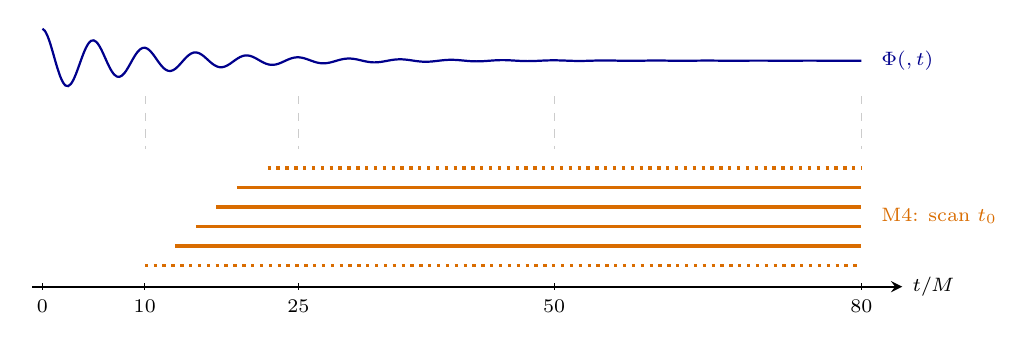
\begin{tikzpicture}[>=stealth, x=0.13cm, y=0.45cm,
                    every node/.style={font=\scriptsize}]
  % --- representative ringdown waveform (top band) ---
  \begin{scope}[yshift=2.6cm]
    \draw[domain=0:80, samples=320, smooth, thick, blue!55!black]
      plot (\x, {0.9*exp(-0.09*\x)*cos(72*\x)});
    \node[blue!55!black, anchor=west] at (81,0)
         {$\Phi(\xq,t)$};
    % light dashed connector to indicate same time axis
    \foreach \x in {10,25,50,80}
      \draw[gray!40, dashed, very thin] (\x,-1.0) -- (\x,-2.5);
  \end{scope}

  % --- M4 windows: vary t_0 in [10,25], fixed t_end = 80 ---
  % plateau block (t_0 = 13..20) drawn solid
  \foreach \t/\y in {13/0.55, 15/1.10, 17/1.65, 19/2.20}
    \draw[orange!85!black, very thick] (\t,\y) -- (80,\y);
  % windows outside the plateau drawn dotted
  \foreach \t/\y in {10/0, 22/2.75}
    \draw[orange!85!black, very thick, dotted] (\t,\y) -- (80,\y);
  \node[orange!85!black, anchor=west] at (81,1.4)
       {M4: scan $t_0$};

  % time axis
  \draw[->, thick] (-1,-0.6) -- (84,-0.6) node[right]{$t/M$};
  \foreach \x in {0,10,25,50,80}
    \draw (\x,-0.5) -- (\x,-0.7) node[below]{$\x$};
\end{tikzpicture}
\caption{M4 schematic: 1-D scan of the start time $t_0$ (six
representative windows of the sixteen-window, step-$1\,M$ scan
shown) with the end time fixed at the usable-signal cutoff
$t=80\,M$. Solid bars belong to the contiguous plateau block and
dotted bars sit outside it. The curve at the top shows a
representative damped waveform on the same time axis.}
\label{fig:m4}
\end{subfigure}

\vspace{1.0em}

%-------------------------------------------------------------
% (b) M5 2-D plateau in (t_0, t_end) plane
%-------------------------------------------------------------
\begin{subfigure}[t]{\textwidth}
\centering
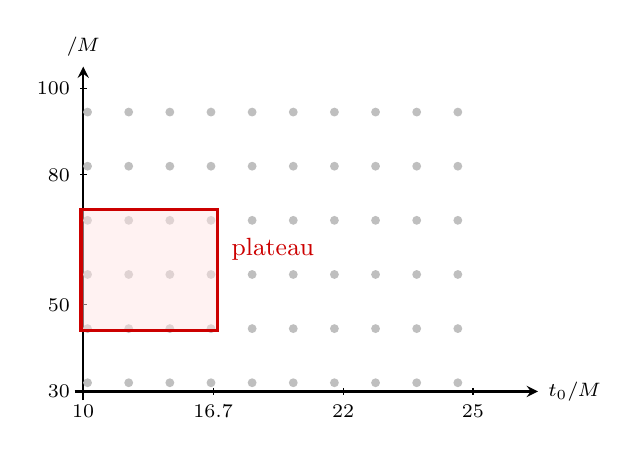
\begin{tikzpicture}[>=stealth, x=0.55cm, y=0.55cm,
                    every node/.style={font=\scriptsize}]
  % axes
  \draw[->, thick] (-0.2,0) -- (10.5,0) node[right]{$t_0/M$};
  \draw[->, thick] (0,-0.2) -- (0,7.5) node[above]{$\tend/M$};
  \foreach \x/\lab in {0/10, 3/16.7, 6/22, 9/25}
    \draw (\x,0.08) -- (\x,-0.08) node[below]{$\lab$};
  \foreach \y/\lab in {0/30, 2/50, 5/80, 7/100}
    \draw (0.08,\y) -- (-0.08,\y) node[left]{$\lab$};

  % grid of (t_0,t_end) candidate windows (10x6 dots)
  \foreach \i in {0,...,9}
    \foreach \j in {0,...,5}
      \fill[gray!50] ({\i*0.95+0.1},{\j*1.25+0.2}) circle (1.6pt);

  % plateau rectangle: t_0 in [10,16.7], t_end in [44,72]
  \draw[red!80!black, very thick, fill=red!10, fill opacity=0.5]
        (-0.05,1.4) rectangle (3.1,4.2);
  \node[red!80!black, anchor=south west, font=\small] at (3.2,2.8)
       {plateau};
\end{tikzpicture}
\caption{M5 schematic: 2-D scan in the $(t_0,\tend)$ plane. Grey
dots are candidate fit windows on a $10\times 6$ grid with
$t_0\in[10,25]\,M$, $\tend\in[30,100]\,M$. The shaded red rectangle
(plateau) is the contiguous $5\times 3$ block of lowest combined
relative scatter measured on the Schwarzschild hFNO waveform,
$t_0\in[10,16.7]\,M$ and $\tend\in[44,72]\,M$.}
\label{fig:m5}
\end{subfigure}
\caption{Fit-window scan schematics for the two plateau-based QNM
extraction methods. (a) M4 sweeps the start time only; (b) M5
sweeps both edges, with the plateau identified as a contiguous
rectangle in the $(t_0,\tend)$ plane.}
\label{fig:windows}
\end{figure}

\FloatBarrier

% --------------------------------------------------------------
\subsubsection{Kerr target-mode protocol}
\label{sec:kerr-qnm}

Kerr extraction introduces a mode-identification problem in addition
to fit-window sensitivity. The labelled $(4,2,0)$ pole can become
subdominant to more slowly decaying late-time components, so a valid
fit need not correspond to the mode being evaluated. We therefore
separate candidate generation from mode identification. Within the
extraction procedure, the Leaver pole identifies the labelled mode but
does not replace any fitted value.

\paragraph{Complex estimators.} For the estimator formulas, let $u$
denote hyperboloidal time and $\tau_{\mathrm d}$ the damping time. A
single complex mode has
$\Psi(\scri,u)=A\exp[(-1/\tau_{\mathrm d}-i\omega_R)(u-u_0)]$,
so $\log|\Psi|$ and the unwrapped phase are linear in $u$. The
c$\Phi$ estimator fits these two slopes. cES instead applies the
ESPRIT construction directly to the complex waveform, without a
Hilbert transform.

\begin{algorithm}[H]
\caption{c$\Phi$ complex-phase estimator.}
\label{alg:cphi}
\begin{algorithmic}[1]
\STATE \textbf{Input:} $\Psi(\scri,u_j)$ on a window $W$.
\STATE $(\widehat a,\widehat b)\gets
  \arg\min_{a,b}\sum_{j\in W}[\log|\Psi_j|-(a+b u_j)]^2$.
\STATE $(\widehat c,\widehat d)\gets
  \arg\min_{c,d}\sum_{j\in W}
  [\operatorname{unwrap}\arg\Psi_j-(c+d u_j)]^2$.
\STATE \textbf{return}
  $(\widehat\omega_R,\widehat\tau_{\mathrm d})
  =(-\widehat d,-1/\widehat b)$.
\end{algorithmic}
\end{algorithm}

\begin{algorithm}[H]
\caption{cES complex ESPRIT estimator.}
\label{alg:ces}
\begin{algorithmic}[1]
\STATE \textbf{Input:} $\Psi(\scri,u_j)$ on a window $W$ and
       model order $K$.
\STATE $\{z_n,c_n\}_{n=0}^{K-1}\gets\operatorname{ESPRIT}_K(\Psi_W)$
       using Eq.~\eqref{eq:esprit-poles}.
\STATE $(\widehat\omega_{R,n},\widehat\tau_{\mathrm d,n})\gets
  [-\operatorname{Im}\log z_n/\Delta u,
  -\Delta u/\operatorname{Re}\log z_n]$.
\STATE \textbf{return} the physical pole selected below.
\end{algorithmic}
\end{algorithm}

\paragraph{Candidate generation and mode identification.} The Leaver
damping time $\tau_{\mathrm{ref}}$ sets all window scales. Targeted M3
($K=6$) and M4 fits are applied separately to
$\operatorname{Re}\Psi$ and $\operatorname{Im}\Psi$ on a
$3\times3$ grid with
$u_{\mathrm{start}}/\tau_{\mathrm{ref}}\in[2,5]$,
$u_{\mathrm{end}}/\tau_{\mathrm{ref}}\in[7,12]$ and duration at
least $3\tau_{\mathrm{ref}}$; cES scans the same windows with
$K\in\{3,4,5,6\}$. M2 on both field components and c$\Phi$ provide
late-time cross-checks on an $8\times6$ grid with
$u_{\mathrm{start}}/\tau_{\mathrm{ref}}\in[4,9]$ and
$u_{\mathrm{end}}/\tau_{\mathrm{ref}}\in[10,14]$, with an
envelope-slope upper cutoff. Multi-mode fits retain the pole nearest
the labelled Leaver pole, and each scan is reduced to its median
candidate. Candidates more than $12\%$ from
$\omega_{R,\mathrm{ref}}$ are rejected. Complete per-estimator
results are reported in Appendix~\ref{app:kerr-extractors}.
% --------------------------------------------------------------
\subsection{Reporting convention}
\label{sec:reporting}

Ringdown parameter recovery is sensitive to the waveform model, fit
interval and extraction procedure, and frequency and damping time can
exhibit markedly different biases, so averaging across the estimator
suite would combine stable fits with identifiable failures
\citep{Berti2007matched,Isi2021priors}. The reported summaries
therefore give the smallest Leaver error attained for each quantity
and record the best accuracy achieved by the suite, not the expected
performance of a fixed estimator.
No Schwarzschild fit uses Leaver values. For the Schwarzschild summary
statistics, the estimator with the smallest Leaver error is selected
separately for frequency and damping time after extraction. The reproduction
comparison is restricted to M1 and M2, while M4 scatter measures
fit-window sensitivity only.
For Kerr, Leaver values identify the $(4,2,0)$ candidate among
multi-mode fits. After extraction, the candidate with the smallest
frequency error and the candidate with the smallest damping-time error
against Leaver are reported separately. Complete per-estimator results
are given in Appendix~\ref{app:kerr-extractors}, and each reported
quantity identifies the selected estimator.